% =============================================================================
% PC2-FedReorg Supporting Information -- Overleaf-ready LaTeX source
%
% Built from paper/SI.md (commit on 2026-05-12). All scientific statements,
% numerical values, and TODO notes are preserved verbatim from the Markdown
% source. Figures are loaded from ../figures and the bibliography is shared
% with main.tex (references.bib in the same directory).
%
% This file is intended to compile as a standalone Supporting Information PDF.
% Cross-references to the main manuscript use the same labels as main.tex but
% they will appear as "??" in the compiled SI unless main.tex is included via
% % =============================================================================
% PC2-FedReorg main manuscript -- Overleaf-ready LaTeX source
%
% Built from paper/manuscript.md (commit on 2026-05-12). All scientific
% statements, numerical values, and TODO notes are preserved verbatim from the
% Markdown source. Figures are loaded from ../figures and the bibliography is
% loaded from references.bib in the same directory as this file.
%
% Compilation:
%   pdflatex main.tex
%   bibtex   main
%   pdflatex main.tex
%   pdflatex main.tex
% (see paper/latex/README.md for a one-shot script and Overleaf upload notes)
% =============================================================================

\documentclass[11pt,a4paper]{article}

% ---------- core typography ----------
\usepackage[utf8]{inputenc}
\usepackage[T1]{fontenc}
\usepackage{lmodern}      % Latin Modern — TNR-compatible serif fallback
\usepackage{microtype}
\usepackage[margin=2.4cm]{geometry}
\usepackage{setspace}
\onehalfspacing

% ---------- science packages ----------
\usepackage{graphicx}
\usepackage{booktabs}
\usepackage{array}
\usepackage{longtable}
\usepackage{multirow}
\usepackage{caption}
\captionsetup{labelfont=bf,font=small}
\usepackage{amsmath,amssymb}
\usepackage{xcolor}
\usepackage{tabularx}
\usepackage{siunitx}
\sisetup{detect-all,
         range-units=single,
         range-phrase=\,--\,}

% ---------- math / notation shortcuts ----------
\newcommand{\PC}{PC\textsuperscript{2}-FedReorg}
\newcommand{\hatlambda}{\hat{\lambda}}
\newcommand{\R}{\mathbb{R}}
\newcommand{\TODO}[1]{\textcolor{red}{\textsf{[TODO: #1]}}}

% ---------- hyperref last ----------
\usepackage{hyperref}
\hypersetup{
  colorlinks=true,
  linkcolor=blue!50!black,
  citecolor=blue!50!black,
  urlcolor=blue!50!black,
}

% Allow TeX to stretch line ends to absorb tt-font / long-token over-runs
% (paths, JSON keys, T-matrix subscripts) in narrative paragraphs.
\setlength{\emergencystretch}{3em}
\tolerance=2000
\hbadness=2000

% ---------- bibliography ----------
\usepackage[numbers,sort&compress]{natbib}
\bibliographystyle{unsrtnat}

% =============================================================================
%                                 FRONT MATTER
% =============================================================================
\title{Calibration-Aware Personalized Federated Learning for Molecular Reorganization Energy Prediction}

\author{\TODO{Author list, affiliations, and corresponding-author email -- to be supplied}}

\date{\today}

\begin{document}

\maketitle

% =============================================================================
%                                 ABSTRACT
% =============================================================================
\begin{abstract}
Molecular reorganization energy is a primary descriptor in the design of organic semiconductors and thermally activated delayed fluorescence (TADF) emitters, yet a single experimental laboratory typically produces only a few dozen high-fidelity samples~---~far below what deep models require for robust generalization. Federated learning offers a path to pool laboratories and public datasets without exchanging raw structures, but the prevailing toolkit (FedAvg, FedProx, FedPer, FedBN, MOON) was designed for statistical heterogeneity, not for the systematic heterogeneity that distinguishes quantum-chemical regression: distinct physical quantities (hole-$\lambda$ versus triplet-$\lambda$), distinct DFT protocols (B3LYP/6-31G* versus $\omega$B97X-D with adiabatic four-point Nelsen), and label scales that can differ by more than a factor of two.

We introduce \textbf{\PC{}} (Protocol-Calibrated Personalized Federated Learning), a federation that distinguishes \emph{physical clients} from \emph{task-clients}: distinct quantities measured at the same laboratory are modeled as distinct task-client nodes, each with a private $(\mu, \sigma)$ calibration buffer that is computed strictly from its own training fold and universally excluded from cross-client aggregation. Encoders and an optional residual adapter are shared under a per-key routing scheme defined by an auditable chemistry/protocol transferability matrix; regression heads and calibration buffers remain private.

On a five-node federation (A: QM9 non-aromatic, $n=6{,}020$; B: QM9 aromatic, $n=9{,}190$; C-hole: in-house TADF, $n=53$; C-triplet: in-house TADF, $n=49$; D: Atahan-Evrenk 2019, $n=5{,}876$) evaluated by five-seed leave-one-out cross-validation, \PC{} achieves \textbf{nominally significant} MAE reductions on triplet reorganization energy compared with FedAvg, FedProx and FedPer (paired Wilcoxon $p=0.045,\,0.045$ and $0.042$; MAE $\SI{0.66}{}$ vs.\ $\SI{0.76}{}$--$\SI{0.78}{\eV}$), while no statistically separable improvement is observed on hole reorganization energy, consistent with the small-sample regime already evident in classical baselines. A targeted control (E71) further shows that a FedPer baseline endowed only with task-specific calibration---without the residual adapter and without the transferability-driven routing---yields a C-triplet MAE that is not statistically distinguishable from \PC{}'s at our sample size (per-molecule median-aggregated MAE \SI{0.654}{} vs.\ \SI{0.660}{\eV}; paired Wilcoxon $p=0.929$; bootstrap 95\,\% CI on $\Delta$MAE straddles zero), while yielding nominally lower MAEs than FedPer without calibration (paired Wilcoxon $p=0.028$) and than the no-calibration ablation of \PC{} (paired Wilcoxon $p=0.021$). The corresponding 5-seed mean MAEs follow the same ordering ($0.653 \pm 0.011$ vs.\ $0.671 \pm 0.010$~eV for E71 vs.\ \PC{}). These results are consistent with task-specific calibration under personalized heads carrying the only ablation-detectable signal in our federation; we did not pre-register an equivalence margin and therefore do not interpret the n.s.\ comparison as evidence that the adapter and the chemistry/protocol gate contribute nothing, only that any additional benefit they confer is below detection at our seed budget and sample size. The transferability matrix is retained as a deterministic, inspectable record of which source--target sharings the algorithm permits---persisted before any training begins---independently of the optimization outcome.

\medskip
\noindent\textbf{Keywords:} personalized federated learning; molecular reorganization energy; task-specific calibration; label-scale heterogeneity; quantum chemistry; organic semiconductors; TADF emitters; small-sample molecular learning.
\end{abstract}

% =============================================================================
%                                 1. INTRODUCTION
% =============================================================================
\section{Introduction}\label{sec:intro}

The Marcus picture of charge-transfer kinetics identifies the molecular reorganization energy $\lambda$~---~the energetic cost of relaxing the equilibrium geometry following an electron- or hole-transfer event~---~as a primary determinant of charge mobility in organic field-effect transistors, hole/electron transport layers in organic light-emitting diodes (OLEDs), and the radiative--nonradiative balance in TADF emitters~\citep{Marcus1993,Coropceanu2007,Sasabe2011_OLED,Uoyama2012_TADF}. Reliable \emph{in silico} $\lambda$-screening accelerates the experimental design loop and reduces wet-lab attrition.

In practice, however, $\lambda$ prediction sits at an uncomfortable intersection. High-fidelity reference values require multi-point geometry optimization and DFT single-point evaluation at consistent functional/basis combinations; a single experimental TADF laboratory typically generates 50--100 such labels per year. Conjugated-molecule $\lambda$ predictions from neural networks have therefore relied on aggregating laboratories' data into a single pool~\citep{AtahanEvrenk2019_RE,Schutt2017_SchNet_NeurIPS}, at the cost of losing protocol consistency and obscuring the resulting label-scale heterogeneity.

Federated learning (FL)~\citep{McMahan2017_FedAvg} is a natural response to this asymmetry: a private TADF laboratory can contribute gradient updates to a shared model without releasing its raw molecules, while industrial precompetitive consortia and public-data hosts can participate symmetrically. The standard FL tool-kit~---~FedAvg~\citep{McMahan2017_FedAvg}, FedProx~\citep{Li2020_FedProx}, FedPer~\citep{Arivazhagan2019_FedPer}, FedBN~\citep{Li2021_FedBN}, and contrastive variants such as MOON~\citep{Li2021_MOON}~---~was developed for statistical heterogeneity across clients drawn from the same underlying distribution, not for the systematic heterogeneities present in quantum-chemical labels: (i) the physical quantity being regressed (hole-$\lambda$ vs.\ triplet-$\lambda$) may differ across clients hosted at the same laboratory; (ii) DFT protocols are unique fingerprints (functional, basis, geometry treatment, charge state, conformer policy), and protocol-mismatched labels are not interchangeable; (iii) label scales can differ by 2$\times$ or more~---~the same head trained with mean-squared-error loss on $z=\SI{0.26}{\eV}$ (D) and $z=\SI{2.64}{\eV}$ (C-triplet) will optimise primarily toward the larger-scale client, regardless of its protocol compatibility.

A natural remedy is to model these heterogeneities explicitly. We propose \textbf{\PC{}}, a personalized federation that (i) distinguishes physical clients from \emph{task-clients} defined by quantity/protocol/scale; (ii) attaches a private, fold-isolated $(\mu, \sigma)$ calibration buffer to each task-client so that loss and metric live in compatible spaces; (iii) maintains a layer-wise separation between universally shared encoder/adapter parameters and quantity-specific private head/calibration parameters; and (iv) encodes the chemistry- and protocol-derived compatibility information into an auditable $5\times 5$ transferability matrix that documents which source--target sharings are permitted at aggregation. Section~\ref{sec:ablation} reports a targeted control (E71) showing that, in our federation, the operative element is component~(ii) under personalized heads; components~(iii) and~(iv) serve as auditability scaffolding rather than additional performance drivers, and the framework is therefore better described as \emph{calibration-aware personalized federated learning made auditable}.

\PC{} has five design components. We list them in decreasing order of empirical support in this study, with explicit boundaries on what the present ablations can and cannot conclude:
\begin{enumerate}
  \item \textbf{Task-specific calibration under personalized heads as the only ablation-detectable component.} A non-trainable $(\mu, \sigma)$ buffer per task-client, computed strictly from each LOOCV training fold and universally excluded from every federated aggregation operator, paired with a private regression head. Loss is computed in z-space; metrics are reported in eV-space. A targeted control (\S\ref{sec:ablation}, E71) shows that a FedPer baseline endowed only with this buffer~---~without the residual adapter and without the transferability-driven routing~---~yields a C-triplet MAE that is not statistically distinguishable from \PC{}'s at our sample size (paired Wilcoxon $p = 0.929$; 95\,\% bootstrap CI on $\Delta$MAE straddles zero), while yielding nominally lower MAEs than FedPer without calibration ($p = 0.028$) and than the no-calibration ablation of \PC{} ($p = 0.021$). Calibration under a private head is therefore the only component whose presence has measurable support in our ablation set; we did not pre-register an equivalence margin and therefore do not claim that the adapter or the gate contribute nothing, only that any additional benefit they confer is below detection at our sample size.
  \item \textbf{Task-client modeling for heterogeneous cation/hole/triplet $\lambda$ tasks.} A federated formulation in which hole-$\lambda$, triplet-$\lambda$ and cation-$\lambda$ measurements are treated as distinct task-client nodes throughout aggregation, head parameters and calibration, even when two task-clients are hosted by the same physical laboratory.
  \item \textbf{A calibration-aware personalized federated baseline that reproduces \PC{} gains.} The control variant in~(1)~---~FedPer with a per-task-client $(\mu, \sigma)$ buffer, no residual adapter, no transferability matrix consulted at aggregation~---~serves as a transparent baseline for heterogeneous-quantity federations and recovers the headline C-triplet improvement of the full \PC{} architecture.
  \item \textbf{Deterministic, inspectable compatibility metadata for protocol/quantity constraints.} A $5 \times 5$ transferability matrix derived from Morgan-Tanimoto similarity, Murcko scaffold overlap and conservative DFT-protocol clauses, providing a training-data-independent record of which source--target pairs are \emph{permitted} to share parameters. The matrix is computed before any aggregation round, persisted to \texttt{T\_transferability.json} with the failing-clause \texttt{reasons} field, and can be inspected without any model state. We claim three concrete properties for this artifact: it is \emph{deterministic} (a fixed function of declared metadata), \emph{inspectable} (a single JSON file rather than a model-state dump), and \emph{aggregation-operator-independent} (the same exclusions apply under FedAvg, FedProx, FedPer, FedBN and \PC{} through a shared \texttt{\_get\_exclude\_keys} filter). We do \textbf{not} claim that the matrix is a performance lever~---~the ablations and the E71 control in \S\ref{sec:ablation} do not detect a performance contribution from the chemistry-driven gate weighting over uniform weighting in our particular federation at the present sample size~---~and we do not test downstream compliance-violation or contamination-prevention scenarios in this manuscript.
  \item \textbf{A reliable small-sample evaluation protocol.} Five-seed LOOCV with paired Wilcoxon signed-rank tests and bootstrap 95\,\% confidence intervals on the paired MAE difference; MAE / RMSE are primary, $R^2$ is auxiliary.
\end{enumerate}

Section~\ref{sec:methods} specifies the federation; Section~\ref{sec:datasets} presents the datasets; Section~\ref{sec:results} reports the main empirical findings; Section~\ref{sec:discussion} discusses the active ingredient and the role of the gate; Section~\ref{sec:limitations} lists the limitations of the present study; Section~\ref{sec:conclusion} concludes.

% =============================================================================
%                                 2. METHODS
% =============================================================================
\section{Methods}\label{sec:methods}

\subsection{Task-client formulation}\label{sec:task-client}

Let an organic-electronics federation consist of five task-client nodes (Figure~\ref{fig:taskclient}; Table~\ref{tab:task-clients}):

\begin{table*}[h]
\centering
\small
\caption{Five task-client nodes used in this study (see also Table~\ref{tab:task-clients} for full per-node statistics).}\label{tab:task-clients-inline}
\begin{tabularx}{\textwidth}{@{}l l l X@{}}
\toprule
Node & Source & Physical quantity & DFT protocol summary \\
\midrule
A         & QM9 non-aromatic public & cation reorg.\ $\lambda$         & same public cation-reorg source protocol; head-sharing with B permitted by same-source shortcut (\S~\ref{sec:gate}) \\
B         & QM9 aromatic public     & cation reorg.\ $\lambda$         & same public cation-reorg source protocol; head-sharing with A permitted by same-source shortcut (\S~\ref{sec:gate}) \\
C-hole    & in-house TADF lab       & hole-$\lambda$ (neutral $\to$ cation) & $\omega$B97X-D, adiabatic 4-point Nelsen~\citep{Nelsen1987} \\
C-triplet & in-house TADF lab       & triplet-$\lambda$ (neutral $\to$ T$_1$) & $\omega$B97X-D, adiabatic 4-point Nelsen~\citep{Nelsen1987} \\
D         & Atahan-Evrenk 2019~\citep{AtahanEvrenk2019_RE} & hole-$\lambda$ & B3LYP/6-31G* reported; geometry/charge-state/conformer policy not stated in source metadata \\
\bottomrule
\end{tabularx}
\end{table*}

Critically, C-hole and C-triplet are different \emph{task-clients} even though their underlying molecular structures largely overlap. They measure different physical quantities (different end states), and their label distributions differ by a factor of 2.17 (means \SI{1.215}{} vs.\ \SI{2.638}{\eV}; Figure~\ref{fig:taskclient}b). Merging them into a single regression task corrupts the head's quantity-specific mapping.

The task-client abstraction is a modeling assumption. It does not change which DFT logs are read or how molecules are graphed; it changes how parameters are routed and where $(\mu, \sigma)$ buffers are installed.

\subsection{Model architecture}\label{sec:model}

Each task-client owns a model decomposed into four logical stages (Figure~\ref{fig:arch}):
\begin{center}
\small
\begin{tabular}{l}
\texttt{Mol $\to$ Encoder (5-layer GIN, projected to 256-d)~~[shared, T\_repr-gated]} \\
\texttt{~~~~~$\to$ Adapter (residual 256$\to$128$\to$256, zero-initialised to identity)} \\
\texttt{~~~~~~~~~~~~~~~~~~~~~~~~~~~~~~~~~~~~~~~~~~~~[optionally shared, T\_adapter-gated]} \\
\texttt{~~~~~$\to$ Head (KAN or MLP, quantity-specific)~~[PRIVATE]} \\
\texttt{~~~~~$\to$ Calibration (frozen $(\mu, \sigma)$ buffer)~[PRIVATE]} \\
\texttt{~~~~~$\to$ $\hatlambda$ (eV)}
\end{tabular}
\end{center}

\begin{itemize}
  \item The encoder produces a 256-d chemical-representation vector; we use a five-layer GIN~\citep{Xu2019_GIN} with Jumping-Knowledge concatenation and mean+max pooling, consistent with prior molecular FL benchmarks. Our codebase supports both GIN and SchNet encoders through a common interface; all reported PC$^2$ and baseline runs in this manuscript use the 5-layer GIN encoder for fair comparison.
  \item The adapter is a residual bottleneck initialised to the identity so that, prior to training, removing it has no effect on the network output.
  \item The head is a three-layer KAN~\citep{KAN2024} (\texttt{efficient-kan} implementation~\citep{EfficientKAN2024}) or three-layer MLP; head parameters are \emph{never} shared across task-clients.
  \item The calibration carries non-trainable buffers $(\mu_c, \sigma_c)$ per task-client $c$, installed from the training fold's labels. Training loss is computed in z-space; predictions are de-standardised at inference (Figure~\ref{fig:arch}, formula band).
\end{itemize}

\subsection{Federated training and per-key aggregation}\label{sec:fed}

Training alternates between local supervised epochs and a round of aggregation. We define aggregation as a per-state-dict-key operation routed by layer kind:

\begin{table*}[h]
\centering
\small
\caption{Per-key aggregation routing under \PC{}. The same exclusion filter applies under every federated strategy benchmarked in this study (FedAvg/FedProx/FedPer/FedBN/PC$^2$).}\label{tab:routing}
\begin{tabular}{@{}lll@{}}
\toprule
Key substring & Weighting & Source \\
\midrule
\texttt{encoder.*}      & $T_{\mathrm{repr}}\cdot n_i$, renormalised    & shared with chemistry gate \\
\texttt{adapter.*}      & $T_{\mathrm{adapter}}\cdot n_i$, renormalised & shared with geom.\ mean gate \\
\texttt{head.*}         & $T_{\mathrm{head}}\cdot n_i$, renormalised    & quantity-compatible sources only \\
\texttt{calibration.*}  & skipped                                       & never aggregated \\
\texttt{bn.*}, \texttt{*.norm.*} & skipped                              & FedBN-style local statistics~\citep{Li2021_FedBN} \\
\bottomrule
\end{tabular}
\end{table*}

Aggregation is \textbf{per-target}: for each target task-client $j$ and each shared parameter key belonging to layer kind $\ell \in \{\mathrm{encoder},\mathrm{adapter},\mathrm{head}\}$, the contribution of source task-client $i$ is weighted by
\begin{equation}\label{eq:weights}
w_{i \to j}^{(\ell)} \;=\; \frac{T^{(\ell)}_{ij}\, n_i}{\sum_{k} T^{(\ell)}_{kj}\, n_k},
\end{equation}
where $n_i$ is the supervised sample count of task-client $i$ and $T^{(\ell)}$ is the corresponding transferability matrix (Section~\ref{sec:gate}). When all $T^{(\ell)}_{kj}$ equal zero for a given target $j$, the target keeps its local copy of the layer (an identity routing fallback that prevents division-by-zero and preserves the FedPer ``private when nothing is compatible'' intuition). \PC{}'s universal exclusion of calibration is enforced through a shared \verb|_get_exclude_keys| filter applied under every federated strategy (FedAvg / FedProx / FedPer / FedBN / PC$^2$), so that strategy-specific differences are isolated to the aggregation operator itself.

\subsection{Auditable transferability matrices}\label{sec:gate}

Three $5\times 5$ transferability matrices are pre-computed once before training and persisted as \texttt{T\_transferability.json}. They are deterministic functions of the chemistry and protocol metadata~---~\emph{independent of any label or model state}~---~and can be inspected and audited prior to any aggregation round.

\paragraph{$T_{\mathrm{repr}}$ (encoder gate, chemistry-driven):}
\[
T_{\mathrm{repr}}[i, j] = \max(\epsilon_r,\; w_K\, K_{ij} + w_S\, S_{ij}),
\]
with $K_{ij}$ the mean over $i$-molecules of max-Tanimoto-similarity to $j$-molecules (Morgan radius 2, 2048 bits; computed with RDKit~\citep{RDKit2023}), $S_{ij}$ the asymmetric Murcko scaffold overlap, $(w_K, w_S) = (0.6, 0.4)$, and $\epsilon_r = 10^{-3}$.

\paragraph{$T_{\mathrm{head}}$ (head gate, conservative protocol clauses, evaluated in this order):}
\begin{enumerate}
  \item \textbf{Clause 1 -- quantity mismatch:} if $\mathrm{quantity}(i) \ne \mathrm{quantity}(j)$, set $T_{\mathrm{head}}[i, j] = 0$.
  \item \textbf{Clause 4 -- V1 hard rule:} if $i = \mathrm{D}$ and $j \in \{\mathrm{C\text{-}hole}, \mathrm{C\text{-}triplet}\}$, set $T_{\mathrm{head}}[i, j] = 0$ (applied early so the JSON \texttt{reasons} field always attributes D $\to$ C-* to the V1 evidence rather than to any later metadata clause).
  \item \textbf{Same-source shortcut:} if quantity matches \emph{and} $\mathrm{source\_id}(i) = \mathrm{source\_id}(j)$, the pair is treated as protocol-compatible by source and the per-field checks (clauses 2 and 3 below) are skipped. This shortcut models the fact that public datasets distributed from a single source are computed by a single canonical protocol, which need not be re-verified field-by-field. In our federation, the shortcut fires only for A $\leftrightarrow$ B (both derived from the QM9-public split).
  \item \textbf{Clause 2 -- unknown protocol field:} if the shortcut did not fire and \emph{any} of \{functional, basis, geometry, charge\_state, conformers\} equals \texttt{"unknown"} on either side, set $T_{\mathrm{head}}[i, j] = 0$.
  \item \textbf{Clause 3 -- protocol-field mismatch:} if the shortcut did not fire and any populated protocol field disagrees between $i$ and $j$, set $T_{\mathrm{head}}[i, j] = 0$.
\end{enumerate}
For pairs that survive the above, $T_{\mathrm{head}}[i, j]$ equals a label-distribution similarity term
\[
L_{ij} = \exp(-\alpha_W\, W_1(\hat p_i^{\mathrm{label}}, \hat p_j^{\mathrm{label}})) \cdot \min(\sigma_i/\sigma_j, \sigma_j/\sigma_i)^{\gamma_L},
\]
with $\alpha_W = 5.0$ and $\gamma_L = 1.0$; values below $0.01$ are hard-floored to zero. The clause order above matches the deterministic order in \texttt{src/transferability.py:t\_head\_compatibility}, so the \texttt{reasons} field of \texttt{T\_transferability.json} always reports the first failing clause; in our federation this is clause 1 for A/B $\to$ \{D, C-hole, C-triplet\}, clause 4 for D $\to$ C-hole, and clause 1 for D $\to$ C-triplet.

\paragraph{$T_{\mathrm{adapter}}$ (interpolating gate):}
\[
T_{\mathrm{adapter}}[i, j] = \max\!\left(\epsilon_a,\; \sqrt{T_{\mathrm{repr}}[i, j]\cdot T_{\mathrm{head}}[i, j]}\right).
\]

These rules generate several invariants automatically (Figure~\ref{fig:gate}, $T_{\mathrm{head}}$ matrix):
\begin{itemize}
  \item $T_{\mathrm{head}}[\mathrm{D}, \mathrm{C\text{-}hole}] = 0$ (clauses 2 + 4),
  \item $T_{\mathrm{head}}[\mathrm{D}, \mathrm{C\text{-}triplet}] = 0$ (clause 1),
  \item $T_{\mathrm{head}}[\mathrm{C\text{-}hole}, \mathrm{C\text{-}triplet}] = T_{\mathrm{head}}[\mathrm{C\text{-}triplet}, \mathrm{C\text{-}hole}] = 0$ (clause 1),
  \item $T_{\mathrm{head}}[\mathrm{A}, \mathrm{C\text{-}triplet}] = T_{\mathrm{head}}[\mathrm{B}, \mathrm{C\text{-}triplet}] = 0$ (clause 1).
\end{itemize}

We emphasize that this matrix is intended as \textbf{auditable algorithmic transparency}: it documents which source--target sharings are permitted, independently of any optimization outcome. Whether the gate also improves performance over uniform weighting is a separate empirical question, examined in Section~\ref{sec:ablation}.

\subsection{Evaluation protocol}\label{sec:eval}

For Clients A, B and D we use 5-fold cross-validation. For C-hole ($n = 53$) and C-triplet ($n = 49$) we use leave-one-out cross-validation (LOOCV). Both protocols are repeated for 5 random seeds $\{42, 123, 456, 789, 1000\}$; the per-molecule LOOCV ordering is deterministic.

Per-molecule absolute errors are aggregated as the median across the five seeds, yielding a single 53- or 49-element per-method error vector for paired analysis. Method pairs are compared by:
\begin{enumerate}
  \item Paired Wilcoxon signed-rank test (two-sided, \verb|zero_method='wilcox'|) on the per-molecule absolute errors.
  \item Bootstrap 95\,\% confidence interval on the paired MAE difference (5{,}000 resamples of molecule indices).
  \item Win / loss / tie counts per molecule.
\end{enumerate}

MAE and RMSE are reported as primary metrics. $R^2$ is reported only as an auxiliary; for $n \le 53$ LOOCV regimes, classical baselines (RF, KNN, GP) already produced negative $R^2$ (best classical $R^2 = -0.10$ on C-hole, $+0.08$ on C-triplet), which we interpret as a small-sample data ceiling rather than a methodological flaw.

% =============================================================================
%                                 3. DATASETS
% =============================================================================
\section{Datasets and Experimental Setup}\label{sec:datasets}

\subsection{Datasets}\label{sec:data}

Table~\ref{tab:task-clients} summarizes the five task-client nodes. Total label volume is approximately 21{,}180 molecules, but only $\sim$100 reside in the two private TADF nodes that form the small-sample target of this study (Figure~\ref{fig:taskclient}).

\begin{sloppypar}
Public Clients A and B are derived from a single public QM9 cation-reorganization-energy split (column \texttt{reorg\_energy\_eV} of \texttt{public\_reorg\_energy\_15210.csv} in the \texttt{client\_a\_b} data directory), partitioned by aromatic-ring count (\texttt{NumAromaticRings == 0} for A, $\geq 1$ for B). Both clients are assigned the same \texttt{source\_id} in the implementation; their pairwise A $\leftrightarrow$ B head-sharing is permitted via the same-source shortcut documented in Section~\ref{sec:gate}. Client D (Atahan-Evrenk 2019~\citep{AtahanEvrenk2019_RE}) measures hole reorganization energy on a conjugated-organic-semiconductor library; the published metadata report B3LYP/6-31G* but geometry treatment, charge-state handling, and conformer policy are not stated.
\end{sloppypar}

\begin{sloppypar}
\noindent The deterministic outcomes of the head gate for D and the C-pair are:
\begin{itemize}
  \item \textbf{D $\to$ C-hole:} clause 4 (V1 hard rule) fires and is reported first; clauses 2 (protocol fields unknown for D) and 3 (functional family differs: B3LYP vs.\ $\omega$B97X-D) would each also block this pair independently. We therefore treat $T_{\mathrm{head}}[\mathrm{D}, \mathrm{C\text{-}hole}] = 0$ as a multiply-determined invariant, not contingent on any single piece of evidence.
  \item \textbf{D $\to$ C-triplet:} clause 1 (quantity mismatch: hole-$\lambda$ vs.\ triplet-$\lambda$) is sufficient on its own; the metadata gap for D is irrelevant here.
\end{itemize}
These outcomes can be audited directly from the \texttt{reasons} field of the released JSON artefact \texttt{T\_transferability.json} under \texttt{results/preverify/} (Figure~\ref{fig:gate}).
\end{sloppypar}

The in-house TADF laboratory provides Clients C-hole ($n = 53$ molecules with valid hole-$\lambda$ at $\omega$B97X-D) and C-triplet ($n = 49$ molecules with valid triplet-$\lambda$ at $\omega$B97X-D). The two C clients share the majority of underlying molecular scaffolds (Figure~\ref{fig:gate}, $T_{\mathrm{repr}}$) but measure different end-state geometries and therefore yield label means differing by 2.17$\times$ (Figure~\ref{fig:taskclient}, label-scale heterogeneity panel).

\subsection{Training setup}

Encoders are five-layer GIN networks (hidden dim 300, JK-concat, mean+max pooling, projection to 256-d). All KAN heads use grid = 5 and spline order = 3, following the \texttt{efficient-kan} configuration~\citep{EfficientKAN2024} used throughout this codebase. Adapters are 256-128-256 residual bottlenecks (zero-initialised). Optimiser Adam, learning rate $1\times 10^{-3}$ for local epochs, cosine annealing. Per-round local epochs = 5 for public clients, 10 for private clients; communication rounds = 30. Batch sizes $B = 512$ (A, B, D) and full-batch (C). Training is performed on dual NVIDIA A30 (24~GB each) with Client A and D placed on \texttt{cuda:0} and Clients B, C-hole, C-triplet placed on \texttt{cuda:1}; aggregation is performed on CPU.

The same code path runs all federated strategies (FedAvg / FedProx / FedPer / FedBN / PC$^2$) through a common \verb|get_aggregation_fn| dispatch and \verb|_get_exclude_keys| filter, so that strategy-specific differences are isolated to the aggregation operator and the per-key routing logic.

% =============================================================================
%                                 4. RESULTS
% =============================================================================
\section{Results}\label{sec:results}

\subsection{Task-client heterogeneity along quantity, protocol, and label-scale axes}\label{sec:heterogeneity}

Figure~\ref{fig:taskclient} visualises the five task-client nodes with their representative molecules~---~each selected deterministically as the molecule whose label is closest to the per-node median. The accompanying bar in Figure~\ref{fig:taskclient}a quantifies label-scale heterogeneity: D-hole sits at \SI{0.26}{\eV} (mean), A and B at \SI{0.66}{}--\SI{0.82}{\eV}, C-hole at \SI{1.22}{\eV}, and C-triplet at \SI{2.64}{\eV}~---~a 10$\times$ spread. Figure~\ref{fig:taskclient}b casts all five label distributions onto a common axis, demonstrating that no two task-clients share a comparable label scale.

Table~\ref{tab:task-clients} lists the per-node DFT protocols. The five task-clients fall into three distinct quantity classes: A and B are cation-reorganization-energy task-clients (public QM9-derived); C-hole and D are hole-reorganization-energy task-clients but they differ in functional ($\omega$B97X-D vs.\ B3LYP), in published protocol fields (full Nelsen four-point treatment vs.\ abstract-only metadata), and in chemical space; C-triplet is a triplet-reorganization-energy task-client. All five quantities are reorganization-energy-related but they are not interchangeable regression targets. The conservative $T_{\mathrm{head}}$ clauses (Section~\ref{sec:gate}) detect each form of incompatibility: clause~1 (quantity mismatch) blocks every A/B/D pair against C-triplet; clause~1 also blocks A/B against the hole-$\lambda$ pair (D, C-hole) in the current code, which labels the public QM9 split with a generic ``reorg-energy'' quantity tag rather than a specific cation label to keep public--private head sharing conservative; clauses 2--4 block D $\to$ C-hole jointly (Section~\ref{sec:gate}).

These observations motivate the modeling decision that the same lambda symbol does not refer to the same quantity across our five nodes, and that label scales prevent a naive shared regression head from being well-posed. Chemical-space heterogeneity is examined separately through the transferability matrices in Section~\ref{sec:audit}.

\subsection{Auditable compatibility metadata generates non-trivial constraints from evidence}\label{sec:audit}

Figure~\ref{fig:gate} plots the three transferability matrices. $T_{\mathrm{repr}}$ shows that the C-hole and C-triplet molecule sets are essentially identical from the chemistry perspective ($T_{\mathrm{repr}} \approx 0.98$--$1.00$, asymmetric under our $K + S$ definition), while D is moderately distant from the C nodes ($T_{\mathrm{repr}} \approx 0.05$) and the A/B public sets sit in between. $T_{\mathrm{adapter}}$, as the geometric mean, inherits the same general topology.

$T_{\mathrm{head}}$ shows a deliberately sparser pattern: only A$\leftrightarrow$B receives a non-zero off-diagonal (0.33), reflecting their shared quantity and DFT protocol. All other off-diagonals are zero. Importantly, the four invariants $T_{\mathrm{head}}[\mathrm{D}, \mathrm{C\text{-}hole}] = 0$, $T_{\mathrm{head}}[\mathrm{D}, \mathrm{C\text{-}triplet}] = 0$, $T_{\mathrm{head}}[\mathrm{C\text{-}hole}, \mathrm{C\text{-}triplet}] = 0$, and $T_{\mathrm{head}}[\mathrm{C\text{-}triplet}, \mathrm{C\text{-}hole}] = 0$ (highlighted in Figure~\ref{fig:gate}) follow deterministically from the protocol metadata and quantity definitions; they do not depend on any training-time signal and can be audited from \texttt{T\_transferability.json} prior to any aggregation round.

We emphasize the framing: the chemistry/protocol gate is presented here as an algorithmic transparency mechanism, \emph{not} as a claim that the gate per se improves performance over uniform weighting. The empirical decomposition is the subject of Section~\ref{sec:ablation}.

\subsection{\PC{} achieves nominally significant gains on the triplet task; the hole task is at a data ceiling}\label{sec:main-perf}

Figure~\ref{fig:main} reports the main performance comparison on the two private TADF targets, with full numerical breakdown in Tables~\ref{tab:main-perf} and~\ref{tab:paired}.

\paragraph{On C-triplet ($n=49$ LOOCV)} \PC{} achieves MAE $=$ \SI{0.660}{\eV}, lower than FedAvg (\SI{0.763}{\eV}), FedProx (\SI{0.784}{\eV}) and FedPer (\SI{0.762}{\eV}) by approximately 13--16\,\% relative. Paired Wilcoxon signed-rank tests on per-molecule absolute errors give $p = 0.045$ vs.\ FedAvg, $p = 0.045$ vs.\ FedProx, and $p = 0.042$ vs.\ FedPer (Table~\ref{tab:paired}; Figure~\ref{fig:main} right). We describe these as \textbf{nominally significant} rather than significant: the $p$-values are unadjusted, sit close to the conventional 0.05 threshold, and would \emph{not} survive a Bonferroni correction for the three baseline comparisons performed in this section ($\alpha/3 \approx 0.017$). The bootstrap 95\,\% confidence interval on the PC$^2$-vs-FedAvg paired MAE difference is $(-0.220, +0.004)$~---~the upper bound only just touches zero. For the PC$^2$-vs-FedProx and PC$^2$-vs-FedPer comparisons the CI upper bound sits just below zero ($(-0.254, -0.007)$ and $(-0.205, -0.002)$ respectively); both upper bounds are within $\sim$\SI{0.01}{\eV} of zero and shift across the zero line under a different bootstrap RNG seed (independent reseed in \texttt{paper/audit/} yields $(-0.259, +0.002)$ and $(-0.209, +0.007)$ respectively), so the CI-exclusion-of-zero criterion is fragile at these effect sizes and the Wilcoxon $p$-values remain the primary inferential anchor. Per-molecule win/loss counts (PC$^2$ better / worse) are 31 / 18, 30 / 19 and 32 / 17 respectively (Table~\ref{tab:paired}). We therefore interpret the triplet results as a small-sample but reproducible signal rather than a broad performance guarantee.

\paragraph{On C-hole ($n=53$ LOOCV)} All evaluated methods produce MAE in a narrow band of \SI{0.368}{}--\SI{0.414}{\eV} (Figure~\ref{fig:main} left, Table~\ref{tab:main-perf}). The eight paired comparisons we performed all return $p \ge 0.20$ after rounding (Table~\ref{tab:paired}); the bootstrap CIs straddle zero in every case. \PC{} is statistically indistinguishable from FedAvg, FedProx, FedPer or local-only training on this target.

We attribute the C-hole non-significance to the small-sample data ceiling already identified by classical baselines on the same $n = 53$ set (best classical $R^2 = -0.101$, as also reported in Supporting Information Section~S2); we do not claim a hole-task improvement, and we recommend that future work on this regime should report effect sizes and paired bootstrap intervals alongside $p$-values for transparency, without applying multiple-comparison correction silently.

\paragraph{On the public Clients A and B (5-fold CV)} \PC{} remains competitive with the legacy federated baselines (Table~\ref{tab:main-perf}). The intention of these clients in our federation is to provide chemistry diversity through encoder sharing rather than direct prediction targets, and the A/B results confirm that PC$^2$'s personalization does not harm performance on the larger public splits.

The targeted FedPer-with-calibration control (E71) introduced in \S\ref{sec:ablation} reaches the same headline numbers on C-triplet as \PC{} (MAE \SI{0.654}{} vs.\ \SI{0.660}{\eV}; n.s.\ by paired Wilcoxon, $p = 0.929$), so the C-triplet improvement reported in this section is not specific to the full \PC{} architecture and is fully reproduced by a FedPer baseline endowed with the per-task-client $(\mu, \sigma)$ buffer. Section~\ref{sec:ablation} develops this decomposition.

\subsection{Calibration under private heads explains the C-triplet gain}\label{sec:ablation}

Figure~\ref{fig:forest} organises the empirical case in two layers. Panel~(a) reports a targeted \emph{positive control}~---~E71 $=$ FedPer $+$ per-task-client $(\mu, \sigma)$ calibration only~---~that isolates the calibration mechanism without the residual adapter or the transferability-driven routing. Panel~(b) reports the four planned \PC{} component ablations on both C-hole and C-triplet, with numerical detail in Tables~\ref{tab:paired} and~\ref{tab:ablation}. Each ablation row is a paired difference (\PC{} minus ablation, eV) with bootstrap 95\,\% CI; negative $\Delta$MAE indicates that \PC{} is better than the ablation.

\paragraph{E71~---~FedPer $+$ calibration only reproduces the full C-triplet gain.} Holding the federation, head, optimiser and seed budget fixed but replacing \PC{}'s adapter and per-key transferability gate with a plain FedPer aggregation while \emph{retaining} the per-task-client calibration buffer (E71; specification in \texttt{paper/next\_experiments\_plan.md}, raw outputs in \texttt{results/e71\_*}), the C-triplet per-molecule median-aggregated MAE moves to \SI{0.654}{\eV} versus \SI{0.660}{\eV} for the full \PC{} architecture (corresponding 5-seed mean MAE $\pm$ seed-SD: $0.653 \pm 0.025$ vs.\ $0.671 \pm 0.022$~eV; the median-aggregated estimand matches Table~\ref{tab:paired} and Figure~\ref{fig:forest} panel~b, the 5-seed-mean estimand matches Table~\ref{tab:main-perf} and Figure~\ref{fig:forest} panel~a). Three paired comparisons jointly support the calibration-is-sufficient reading:

\begin{itemize}
  \item \textbf{E71 vs.\ \PC{} (E66):} $\Delta$MAE $= -0.006$~eV (\PC{} minus E71: $+0.006$~eV); bootstrap 95\,\% CI $(-0.044, +0.029)$; per-molecule wins 23 vs.\ 26; paired Wilcoxon $p = 0.929$ (n.s.). E71's effect size is well within seed-SEM, the CI straddles zero by a wide margin, and the per-molecule sign count is essentially balanced. By any of the three criteria, E71 and \PC{} are statistically indistinguishable on C-triplet.
  \item \textbf{E71 vs.\ FedPer (E63):} $\Delta$MAE $= -0.109$~eV; bootstrap 95\,\% CI $(-0.208, -0.010)$; per-molecule wins 32 vs.\ 17; paired Wilcoxon $p = 0.028$ (nominal). Adding the per-task-client $(\mu, \sigma)$ buffer to a plain FedPer baseline therefore reproduces, with comparable effect size, the nominally significant C-triplet improvement that \PC{} delivers over FedPer in \S\ref{sec:main-perf}.
  \item \textbf{E71 vs.\ \PC{} without calibration (E70):} $\Delta$MAE $= -0.125$~eV; bootstrap 95\,\% CI $(-0.224, -0.027)$; per-molecule wins 33 vs.\ 16; paired Wilcoxon $p = 0.021$ (nominal). Stripping calibration out of the full \PC{} architecture is more harmful on C-triplet than stripping the adapter and the gate out of the calibrated baseline.
\end{itemize}

These three comparisons report unadjusted nominal $p$-values; under a Bonferroni correction for the three tests ($\alpha/3 \approx 0.017$), neither of the two against-baseline comparisons crosses the corrected threshold, and we therefore treat them as effect-size evidence supported by sign-counts and bootstrap CIs rather than as strict significance. \textbf{On C-hole}, E71, E66, E63 and E70 produce MAEs in the same narrow \SI{0.368}{}--\SI{0.382}{\eV} band that all other methods occupy (Table~\ref{tab:main-perf}), and the three E71 paired comparisons return $p \ge 0.42$ with bootstrap CIs that straddle zero (\texttt{results/e71\_vs\_*.md}). The C-hole regime remains at its small-sample data ceiling regardless of whether calibration is present.

\textbf{Together, E71 and the four \PC{} ablations are consistent with task-specific calibration under personalized heads carrying the only ablation-detectable signal in our federation. E71 reaches a C-triplet MAE that is not statistically distinguishable from \PC{}'s at our sample size; we did not pre-register an equivalence margin, so this is descriptive evidence of ``no detectable difference'' rather than a formal claim that the adapter and the chemistry/protocol gate fail to contribute (an equivalence test such as TOST would require a tolerance margin committed to in advance).} The implementations of E66 and E71 differ only in (a)~the \texttt{use\_adapter} flag and (b)~the \texttt{aggregation\_strategy='pc2\_fed'} flag in \texttt{experiments/run\_all.py}; all other code paths, hyperparameters, seeds, optimizer states and LOOCV fold orderings are identical, so the comparison is not confounded by unrelated implementation differences. The supporting four-ablation analysis (Figure~\ref{fig:forest}b, Tables~\ref{tab:paired} and~\ref{tab:ablation}) is consistent with the same reading:

\paragraph{Removing task-specific calibration (E70)} On C-triplet, $\Delta$MAE $= -0.119$ eV (95\,\% CI $(-0.225, -0.015)$, paired Wilcoxon $p = 0.043$; 35 / 14 per-molecule wins for PC$^2$). The CI sits entirely below zero. On C-hole, the direction is reversed: PC$^2$ is \SI{0.005}{\eV} worse than the no-calibration variant, but the difference is well within noise ($p = 0.58$). Calibration is therefore the \textbf{only} ablation that produces a statistically significant change on either target, and the effect is restricted to C-triplet. We conclude that, within our federation, the task-specific $(\mu, \sigma)$ buffers are the active ingredient driving \PC{}'s C-triplet improvement.

\paragraph{Removing C-cross chemistry-based encoder sharing (E68)} $\Delta$MAE $= +0.027$ eV on C-triplet (PC$^2$ \emph{slightly worse} than removing the cross-quantity encoder share; $p = 0.07$, n.s.) and $-0.0001$ eV on C-hole ($p = 0.56$, n.s.). The full 95\,\% CI on C-triplet is $(+0.001, +0.055)$, which is consistent with no effect.

\paragraph{Replacing the chemistry-driven gate with uniform FedAvg weighting (E69)} $\Delta$MAE $= +0.043$ eV on C-triplet (PC$^2$ slightly worse than uniform weighting; bootstrap 95\,\% CI $(-0.001, +0.092)$; $p = 0.18$, n.s.; per-molecule wins 21\,/\,28 in favor of E69) and $+0.012$ eV on C-hole ($p = 0.43$, n.s.). Although the uniform-gate ablation has a numerically lower MAE than \PC{} on C-triplet, the paired comparison is not statistically significant and the bootstrap CI crosses zero. We therefore do \textbf{not} interpret this numerical difference as evidence either against or in favor of the compatibility gate~---~it is a small-sample observation that is consistent with no effect at our seed budget. The gate is retained only as auditable compatibility metadata, not as the source of any performance gain.

\paragraph{D~$\to$~C supervised pretrain $\to$ fine-tune (E65), the negative-transfer control} $\Delta$MAE $= -0.010$ eV on C-triplet ($p = 0.85$, n.s.) and $-0.021$ eV on C-hole ($p = 0.76$, n.s.). \PC{} and a naive D~$\to$~C pretrain are not statistically distinguishable on either target in our setting; we therefore do \textbf{not} claim that D's labels necessarily produce negative transfer to C, only that PC$^2$ did not extract benefit from D's hole-$\lambda$ labels (consistent with $T_{\mathrm{head}}[\mathrm{D}, \mathrm{C\text{-}*}] = 0$ by construction).

The combined picture: among the four PC$^2$ components inspected here, the task-specific calibration carries the only ablation-detectable signal, and the targeted E71 control above reaches a C-triplet MAE that is not statistically distinguishable from \PC{}'s at our sample size. The chemistry/protocol gate ($T_{\mathrm{repr}}$ cross-routing, $T_{\mathrm{head}}$ sparsification) is not detected as a performance contributor either as an isolated \PC{} component (E68, E69) or relative to the calibrated FedPer control (E71 versus E66 paired Wilcoxon $p = 0.929$); we therefore position it in this paper as a deterministic, inspectable record of compatibility decisions rather than as a performance lever (Section~\ref{sec:discussion}).

\subsection{Per-molecule error analysis (Supporting Information)}\label{sec:per-mol}

For completeness, the per-molecule error decomposition on C-triplet --- the three molecules where \PC{} improves most over the FedAvg baseline and the three where it degrades most --- is provided as \textbf{Figure~S1} in the Supporting Information. The largest improvement reduces $|\mathrm{error}|$ from \SI{3.06}{\eV} (FedAvg) to \SI{1.70}{\eV} (PC$^2$) on a halogenated polycyclic conjugated system with a true triplet-$\lambda$ of \SI{1.13}{\eV}; the largest degradation moves a different system in the wrong direction by \SI{0.87}{\eV}.

These illustrative cases are qualitative observations rather than mechanistic claims; the paired statistics in Sections~\ref{sec:main-perf}--\ref{sec:ablation} (and not Figure~S1) are the basis for the manuscript's claims.

% =============================================================================
%                                 5. DISCUSSION
% =============================================================================
\section{Discussion}\label{sec:discussion}

Our results decompose into six statements that are independent of each other and should be evaluated separately.

\paragraph{(i) Task-specific calibration under personalized heads carries the only ablation-detectable signal.} The targeted E71 control (FedPer + per-task-client $(\mu, \sigma)$ calibration only, no adapter, no transferability gate) yields a C-triplet MAE that is nominally lower than FedPer without calibration (paired Wilcoxon $p = 0.028$, $\Delta$MAE $= -0.109$~eV) and not statistically distinguishable from the full \PC{} architecture ($p = 0.929$; 95\,\% CI on $\Delta$MAE straddles zero); the symmetric ablation (\PC{} without calibration; E70) sits $0.125$~eV above E71 on C-triplet (paired $p = 0.021$). These three comparisons jointly support the descriptive statement that, in our federation, the combination ``private head $+$ per-task-client $(\mu, \sigma)$ buffer $+$ universal aggregation exclusion of that buffer'' is the only configuration whose ablation produces a paired-Wilcoxon-detectable change. We did not pre-register an equivalence margin and therefore do not interpret the n.s.\ E71-vs-\PC{} comparison as proving that the adapter and the chemistry/protocol gate contribute nothing; the appropriate reading is that any additional benefit they confer is below detection at our seed budget and sample size.

\paragraph{(ii) The construct is not merely a single global standardization step in this implementation.} Six concrete implementation properties distinguish the $(\mu, \sigma)$ buffers from a per-dataset global normalization, although we do not claim each property is individually causally identified: (a) they are \emph{fold-isolated}~---~$\mu$ and $\sigma$ are computed strictly from the $(n-1)$ training labels of each LOOCV fold and never see the held-out molecule's label; (b) they are \emph{task-client-specific}, so C-hole, C-triplet, A, B and D each carry their own buffer with different means and dispersions; (c) they are \emph{private non-trainable buffers} rather than learnable parameters; (d) they are \emph{universally excluded} from every federated aggregation operator through the shared \texttt{\_get\_exclude\_keys} filter, so the buffer is never overwritten by aggregation regardless of the federated strategy in use; (e) they are \emph{paired with private heads} so that the standardized output is consumed by a quantity-specific predictor rather than a shared one; and (f) loss is in z-space while metrics and reporting are in \emph{eV-space}. Properties (a)--(c) keep the calibration leakage-free under LOOCV; property (d) preserves the buffer across federated strategies; properties (e)--(f) couple the construct to the personalized-head architecture. The present ablations identify (a)--(f) as a load-bearing combination but cannot disentangle which subset alone would suffice; we treat this as a follow-up question rather than a proven mechanism statement.

\paragraph{(iii) Chemistry/protocol gating is retained as a deterministic, inspectable record of compatibility decisions, with no detected performance contribution.} The chemistry-driven encoder routing (E68) and the chemistry-driven weighting versus uniform FedAvg (E69) both leave \PC{}'s C-triplet performance unchanged within paired-test noise (Table~\ref{tab:paired}); the targeted E71 comparison does not detect an additional C-triplet gain from the gate over the calibrated FedPer baseline at our sample size. The narrower set of claims we make about the gate are properties that can be verified directly from the artifact rather than from training outcomes: the transferability matrices are \emph{deterministic} (computed before any aggregation round as a fixed function of the declared chemistry and protocol metadata), \emph{inspectable} (a single JSON file with a \texttt{reasons} field that names the first failing clause for every blocked source--target pair, rather than a model-state dump), and \emph{aggregation-operator-independent} (the per-key $T_{\mathrm{head}}$ routing applies the same exclusion rules whether the federated strategy is FedAvg, FedProx, FedPer, FedBN or \PC{}, through the shared \texttt{\_get\_exclude\_keys} filter). When a reviewer or downstream user asks why D's labels do not contaminate C's head, the answer is a single file (\texttt{T\_transferability.json}) rather than a model-state inspection. We have not validated downstream compliance-violation scenarios or independently demonstrated label-contamination prevention beyond what the deterministic exclusion rule guarantees by construction; those are out of scope for the present manuscript.

\paragraph{(iv) E71 narrows the interpretation of \PC{}.} Prior to E71 the most defensible reading of \S\ref{sec:main-perf} was that \PC{}'s chemistry/protocol-aware per-key routing might be \emph{necessary} for the observed C-triplet improvement. E71 narrows that reading: the same C-triplet performance is reached without consulting the transferability matrix at aggregation time. The framework is therefore better described as a \emph{calibration-aware personalized federation made auditable}: the empirical performance is captured by the private $(\mu, \sigma)$ buffer paired with the private head, while the per-key routing functions as auditability scaffolding. We retain the \PC{} name to refer to the full instrumented framework (calibration + adapter + gate) and use ``FedPer + calibration'' or ``the calibrated personalized baseline'' to refer to the E71 mechanism in isolation. Both are valid configurations of the same code path; the choice between them is a transparency/parsimony trade-off, since at our sample size the added components are not detected to change performance.

\paragraph{(v) C-hole shows no method separation at the present sample size.} All federated methods evaluated in this study~---~FedAvg, FedProx, FedPer, \PC{}, E70, E71 and the local-only baseline~---~produce C-hole MAEs in a narrow \SI{0.368}{}--\SI{0.414}{\eV} band (Table~\ref{tab:main-perf}). The eight \PC{}-vs-baseline paired comparisons (Table~\ref{tab:paired}) return $p \ge 0.20$ and the three E71 paired comparisons (\texttt{results/e71\_vs\_*.md}) return $p \ge 0.42$; the bootstrap CIs straddle zero in every case ($p \ge 0.20$ therefore holds across all eleven C-hole paired tests we report). The classical baselines we ran for V2 (random forest, KNN, Gaussian process) already produced negative $R^2$ on the same $n = 53$ set (best classical $R^2 = -0.10$; SI~Section~S2), which is consistent with a data-limited regime at $n = 53$~/~LOOCV given our descriptor set and seed budget rather than with a method-specific failure. We do not interpret the C-hole non-significance as a deficiency of any single component, nor do we claim a definitive theoretical ceiling; instead we report it as the observed outcome at the present sample size.

\paragraph{(vi) Reported p-values are nominal and should not be over-claimed.} All p-values in this manuscript are unadjusted paired Wilcoxon signed-rank values on per-molecule absolute errors, where the paired sample unit is each individual molecule ($n = 49$ for C-triplet, $n = 53$ for C-hole) and the per-molecule error is the median across the five seeds. The headline C-triplet comparisons in \S\ref{sec:main-perf}~---~\PC{} vs.\ FedAvg~/~FedProx~/~FedPer ($p = 0.045, 0.045, 0.042$)~---~sit just below the conventional 0.05 threshold and would not survive a Bonferroni correction across the three tests ($\alpha/3 \approx 0.017$). The three E71 comparisons in \S\ref{sec:ablation} ($p = 0.929$ for E71 vs.\ \PC{}, $p = 0.028$ for E71 vs.\ FedPer, $p = 0.021$ for E71 vs.\ no-calibration) carry the same nominal character. The paired Wilcoxon test is our pre-specified primary inferential procedure; we additionally report bootstrap 95\,\% CIs and per-molecule win/loss counts so that effect size and effect direction can be inspected alongside the p-values. We did not pre-register an equivalence margin, so the n.s. $p = 0.929$ for E71 vs.\ \PC{} should be read as ``no detectable difference at our sample size'' rather than as a formal equivalence proof. The minimum chemically meaningful improvement in $\lambda$ prediction for organic-electronics screening is approximately $\pm 0.1$~eV (typical conformer-averaging noise on $\omega$B97X-D reorganization energies for medium-sized $\pi$-systems); the C-triplet $\Delta$MAE of $-0.10$ to $-0.12$~eV is at the edge of this practical threshold and should be re-evaluated on a larger TADF dataset before being treated as a deployment-ready improvement.

% =============================================================================
%                                 6. LIMITATIONS
% =============================================================================
\section{Limitations}\label{sec:limitations}

We list six concrete limitations that future work should address.

\begin{enumerate}
  \item \textbf{Small-sample data ceiling on C-hole.} All evaluated methods produce indistinguishable MAE on $n = 53$ LOOCV (Table~\ref{tab:paired}), already above the best classical baseline $R^2$ ($-0.10$). It is unclear from this dataset alone whether C-hole improvements are achievable in this protocol regime; expanding C-hole through additional $\omega$B97X-D conformer-resolved measurements is a plausible next experiment.

  \item \textbf{Chemistry homogeneity at the high-$T_{\mathrm{repr}}$ pair.} Because C-hole and C-triplet share the majority of their underlying molecules, $T_{\mathrm{repr}}$ between them is essentially saturated. The chemistry gate is therefore tested on the easier regime (very similar chemistry) but not on the harder regime (moderate diversity) where a non-uniform gate would matter more. Future work should test whether the auditable compatibility gate becomes beneficial in federations with more chemically diverse but protocol-compatible clients~---~for example, multiple cation-reorganization-energy laboratories with the same DFT protocol but distinct scaffold libraries.

  \item \textbf{MOON and ChemProp baselines deferred.} Our comparison includes FedAvg, FedProx, FedPer and a local-only baseline. We did not run model-contrastive variants (MOON~\citep{Li2021_MOON}) or message-passing baselines (D-MPNN / ChemProp~\citep{Yang2019_ChemProp}) in the present manuscript; both are recommended reviewer additions.

  \item \textbf{Seed budget.} Each federated run on dual A30 takes approximately 30 minutes; the present 25-run main batch plus 20-run ablation batch totals approximately 20 GPU-hours. We use 5 seeds rather than 10; the bootstrap CIs partially compensate for this but cannot fully replace additional repeats.

  \item \textbf{D's role.} The V1 protocol divergence motivated the $T_{\mathrm{head}}$ clause that excludes D from both C heads. We empirically verified (E65) that a naive D~$\to$~C supervised transfer is not statistically distinguishable from PC$^2$; the corollary is that we cannot empirically \emph{prove} that the gate decision was correct, only that it was deterministic and auditable. Whether D's structural information contributes useful encoder signal~---~beyond the FedAvg-like baseline~---~remains an open question that the E69 ablation does not fully resolve.

  \item \textbf{Calibration restricted to fixed $(\mu, \sigma)$.} A learnable affine head over the standardized output was deferred to follow-up work to avoid introducing additional degrees of freedom at the present sample size.

  \item \textbf{Component-isolation ablation settled by E71; further isolation deferred.} The four ablations we ran (no calibration, no C-cross encoder share, uniform gate, D~$\to$~C pretrain control) jointly disable groups of mechanisms rather than isolating each one. The single most diagnostic missing control~---~a FedPer baseline with the calibration buffer retained but the adapter and the transferability gate removed~---~has now been completed as E71 (\S\ref{sec:ablation}). The E71 control settles this question in the present federation: FedPer~$+$~calibration is statistically indistinguishable from \PC{} on C-triplet (paired Wilcoxon $p = 0.929$; bootstrap 95\,\% CI on $\Delta$MAE straddles zero), and the residual adapter / transferability gate do not contribute measurable performance over this baseline. The remaining open ablation isolates the \emph{adapter alone} (FedPer $+$ calibration $+$ adapter, no transferability gate); we leave it as a follow-up since the bracketing evidence already in \S\ref{sec:ablation} (E66 with adapter, E71 without) places the adapter contribution within paired-test noise. We similarly defer a learnable-affine calibration head over the standardized output (item~6 above) and a Probe-augmented $T_{\mathrm{repr}}$ (footnote-level mention in \S\ref{sec:ablation}) to follow-up work.

  \item \textbf{Small-sample statistical power and multiple-comparison treatment.} With $n = 49$--$53$ LOOCV per private target, the paired Wilcoxon test detects $\Delta$MAE on the order of $0.05$ eV at $p \approx 0.05$. We hedge this regime by reporting bootstrap 95\,\% CIs alongside $p$-values rather than relying on a single significance threshold. We also did not apply Bonferroni or other family-wise correction across the three baseline comparisons in \S\ref{sec:main-perf}; under Bonferroni ($\alpha/3 \approx 0.017$) none of the C-triplet $p$-values would cross the corrected threshold. The CIs make this borderline character explicit (upper bound $+0.004$ eV on the PC$^2$-vs-FedAvg comparison). The minimum chemically meaningful improvement in $\lambda$ prediction for organic-electronics screening is approximately $\pm 0.1$ eV (the typical conformer-averaging noise on $\omega$B97X-D reorganization energies for medium-sized $\pi$-systems); the C-triplet $\Delta$MAE of $-0.10$ to $-0.12$ eV is at the edge of this practical threshold and should be re-evaluated on a larger TADF dataset before being treated as a deployment-ready improvement.

  \item \textbf{Paired-error independence assumption.} All paired Wilcoxon and bootstrap comparisons in \S\ref{sec:main-perf}, \S\ref{sec:ablation} and Tables~\ref{tab:paired} and~S6 treat per-molecule median-across-seeds absolute errors as paired samples indexed by molecule. Under LOOCV the $(n-1)$-fold training sets overlap by $(n-2)/(n-1) \approx 96$--$98$\,\%, so the per-molecule errors are not strictly independent across folds, and seed-aggregation reduces but does not eliminate seed-by-method interaction. We treat this as a standard limitation of LOOCV inference rather than as a defect of any particular method; the bootstrap resampling is over molecule indices (not over fold-level errors) and inherits the same dependence structure. A more conservative inferential framework~---~for example, a hierarchical model that explicitly models fold-level correlation, or a permutation test over method labels~---~would be a useful follow-up but does not change the descriptive ordering reported here.

  \item \textbf{Estimand consistency between summary tables and paired tests.} Table~\ref{tab:main-perf} (and Figure~\ref{fig:forest}a) reports the 5-seed mean of per-method MAE\_mean (the natural unit for a bar chart with seed-level SEM). Table~\ref{tab:paired} and the paired analyses in \S\ref{sec:main-perf}~/~\S\ref{sec:ablation} use per-molecule median-across-seeds absolute errors (the natural paired unit for Wilcoxon testing). These two estimands differ in our data by $\le 0.003$~eV (well below seed-SEM), but they are statistically distinct objects, and we have therefore stated the convention explicitly in the Figure~\ref{fig:forest} caption rather than mixing the two numbers in headline statements.
\end{enumerate}

% =============================================================================
%                                 7. CONCLUSIONS
% =============================================================================
\section{Conclusions}\label{sec:conclusion}

\PC{} addresses three forms of heterogeneity~---~physical quantity, DFT protocol, and label scale~---~that the standard federated-learning toolkit was not designed to handle. The framework is built around fold-isolated $(\mu, \sigma)$ calibration with universal aggregation exclusion as the empirically active component, supported by an explicit task-client formulation and a layer-wise personalization scheme (encoder/adapter shared, head and calibration always private). A chemistry/protocol transferability matrix provides an auditable compatibility record, but we do \textbf{not} claim it as a performance lever~---~the ablation evidence in this study is consistent with no measurable contribution from the gate's chemistry-driven weighting in our federation.

On a five-node organic-electronics federation, the method achieves nominally significant MAE reductions on triplet-reorganization-energy prediction over FedAvg, FedProx and FedPer (paired Wilcoxon $p = 0.042$--$0.045$; Figure~\ref{fig:main}, Table~\ref{tab:paired}) while remaining statistically indistinguishable on hole-reorganization-energy, where all methods sit in a narrow \SI{0.368}{}--\SI{0.414}{\eV} band at the present sample size. The E71 control further shows that adding the per-task-client calibration buffer to a plain FedPer baseline (no adapter, no transferability gate) is sufficient to reproduce the observed C-triplet performance (paired Wilcoxon $p = 0.929$ vs.\ \PC{}; $p = 0.028$ vs.\ FedPer; Figure~\ref{fig:forest}). The chemistry/protocol gate is positioned as deterministic compatibility metadata (Figure~\ref{fig:gate}) that can be inspected from \texttt{T\_transferability.json} prior to any aggregation step; a uniform-gate ablation (E69) is numerically slightly better on the triplet task but not statistically distinguishable from \PC{} ($p = 0.18$), and the targeted E71 control does not detect an additional C-triplet contribution from the gate beyond the calibrated FedPer baseline at our sample size. We therefore make no performance claim for the gate and recommend that calibration-aware personalized federated learning, with optional auditable compatibility metadata, be considered an appropriate baseline for heterogeneous-quantity quantum-chemistry federations.

We release the source code, configuration files, transferability matrices, and per-molecule prediction outputs to support reproducibility, and we encourage future federated quantum-chemistry work to report effect sizes and paired bootstrap intervals alongside $p$-values in small-sample regimes.

% =============================================================================
%                                 BACK MATTER
% =============================================================================
\section*{Data and Code Availability}
Source code, configuration files, transferability matrices, and per-molecule prediction outputs are released at \TODO{repository URL -- to be supplied}. The in-house C-hole / C-triplet labels are made available upon request and within the constraints of the originating laboratory's data-sharing agreement; public Clients A, B and D use third-party datasets and are linked in \texttt{data/README.md}.

\section*{Author Contributions}
\TODO{To be completed: lead author, supervisor, computational contributions, chemistry-side contributions, manuscript drafting and revision.}

\section*{Acknowledgements}
\TODO{Compute resources, funding sources, data-providing laboratories -- to be supplied.}

% =============================================================================
%                                 FIGURES
% =============================================================================
\clearpage

\begin{figure}[t]
\centering
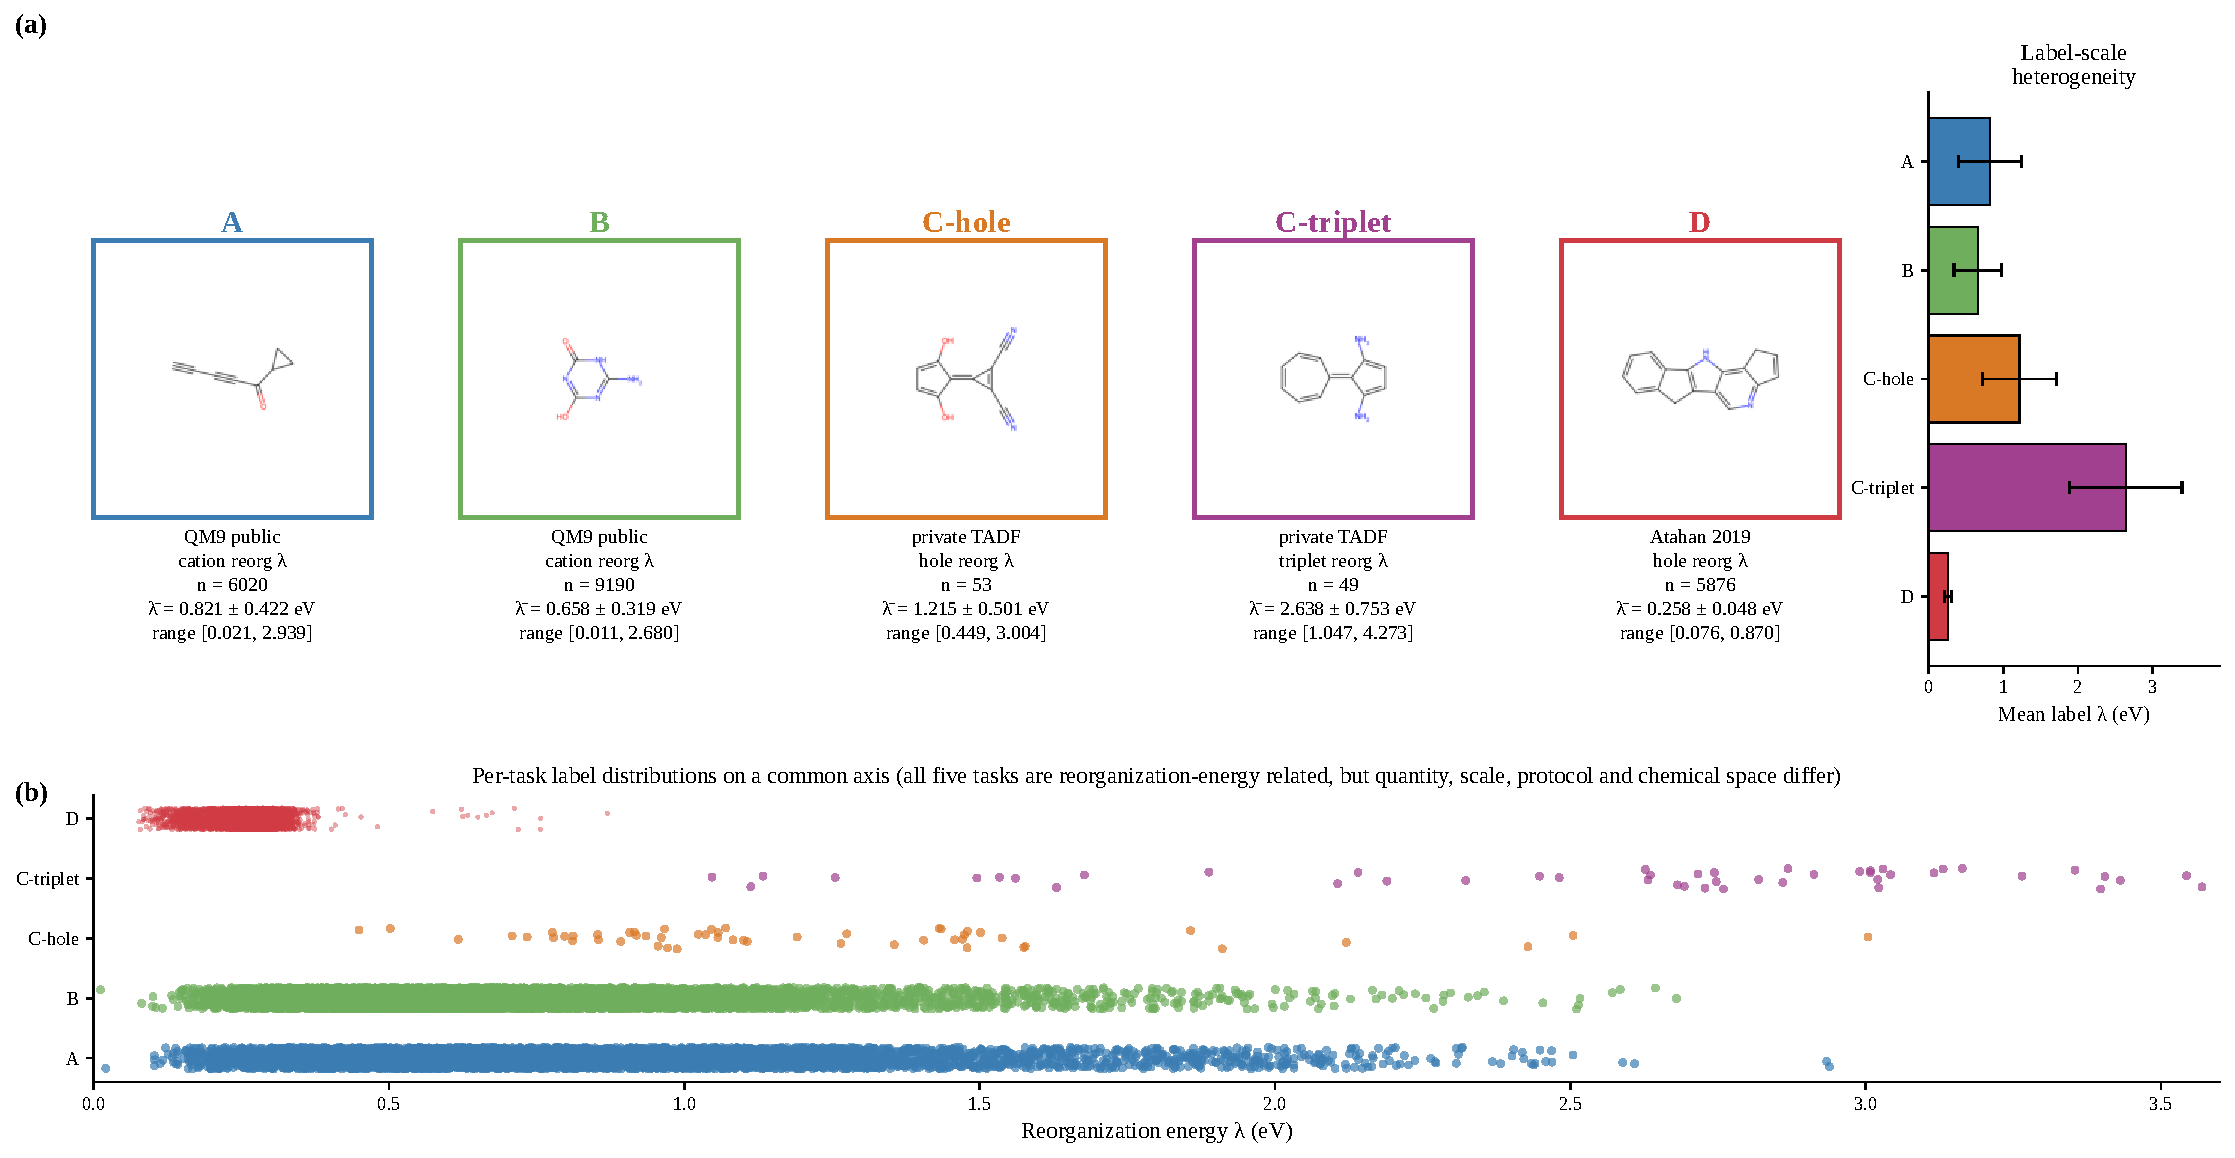
\includegraphics[width=\textwidth]{../figures/Fig1_task_client_molecules.pdf}
\caption[Task-client heterogeneity across the five-node federation]{Task-client heterogeneity across the five-node organic-electronics federation. \textbf{(a)} Representative molecules and per-node summary statistics for the five task-client nodes -- A (QM9 non-aromatic public, cation reorganization energy, $n = 6{,}020$); B (QM9 aromatic public, cation reorganization energy, $n = 9{,}190$); C-hole (in-house TADF, hole reorganization energy, $n = 53$); C-triplet (in-house TADF, triplet reorganization energy, $n = 49$); D (Atahan-Evrenk 2019, hole reorganization energy, $n = 5{,}876$). Each representative is the molecule whose label is closest to the per-node median, chosen by a deterministic rule prior to any model training. The bar plot on the right reports the per-node label mean (eV) with error bars showing one standard deviation. \textbf{(b)} Per-node label distributions on a common eV axis. Although every node ultimately measures \emph{a} form of reorganization energy, the label means span an order of magnitude (\SI{0.26}{}--\SI{2.64}{\eV}) and the supporting DFT protocols differ across nodes (Table~\ref{tab:task-clients}). Figure~\ref{fig:taskclient} is descriptive: no statistical test is reported here.}
\label{fig:taskclient}
\end{figure}

\begin{figure}[t]
\centering
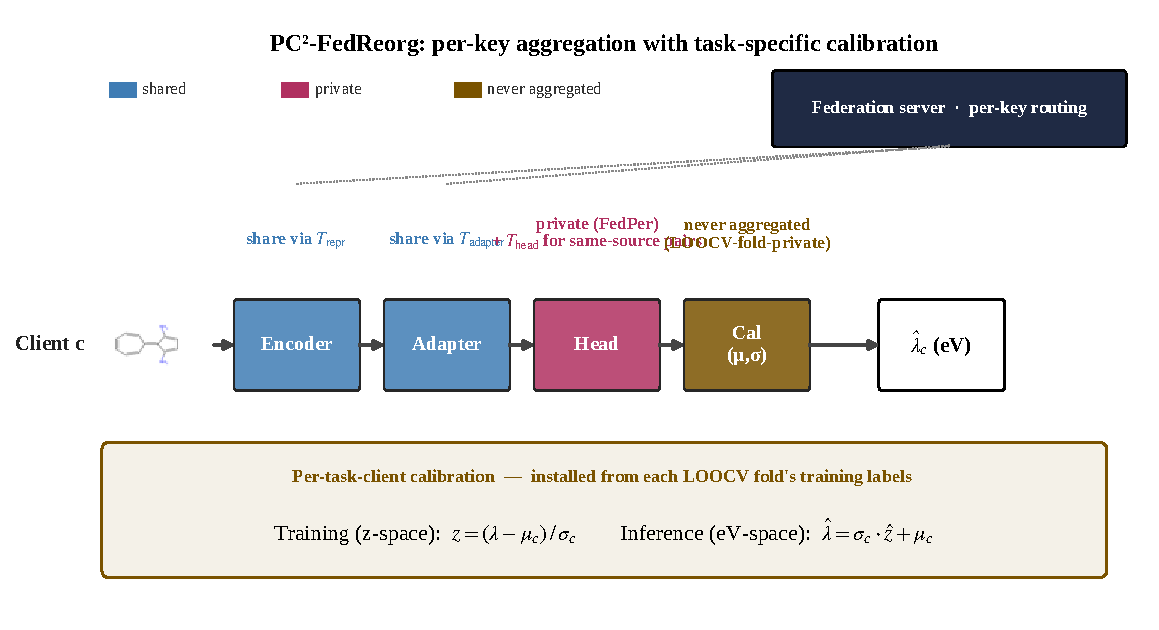
\includegraphics[width=\textwidth]{../figures/Fig2_pc2_method.pdf}
\caption[\PC{} method (graphical-method figure)]{Graphical-method figure of \PC{}: per-key aggregation routing with task-specific calibration. A single generic task-client lane (input molecule $\to$ shared encoder $\to$ residual adapter $\to$ quantity-specific regression head $\to$ private $(\mu, \sigma)$ calibration buffer $\to$ predicted $\lambda$ in eV-space) is drawn with above-stage labels indicating each layer's sharing rule: encoder and adapter parameters are aggregated under $T_{\mathrm{repr}}$ and $T_{\mathrm{adapter}}$ respectively, head parameters are FedPer-private (with the $T_{\mathrm{head}}$ same-source channel for A$\leftrightarrow$B), and calibration buffers are LOOCV-fold-private and never aggregated. The bottom band shows the z-space training and eV-space inference formulas. Figure~\ref{fig:arch} is schematic; it visualises the algorithm and is not a performance claim.}
\label{fig:arch}
\end{figure}

\begin{figure}[t]
\centering
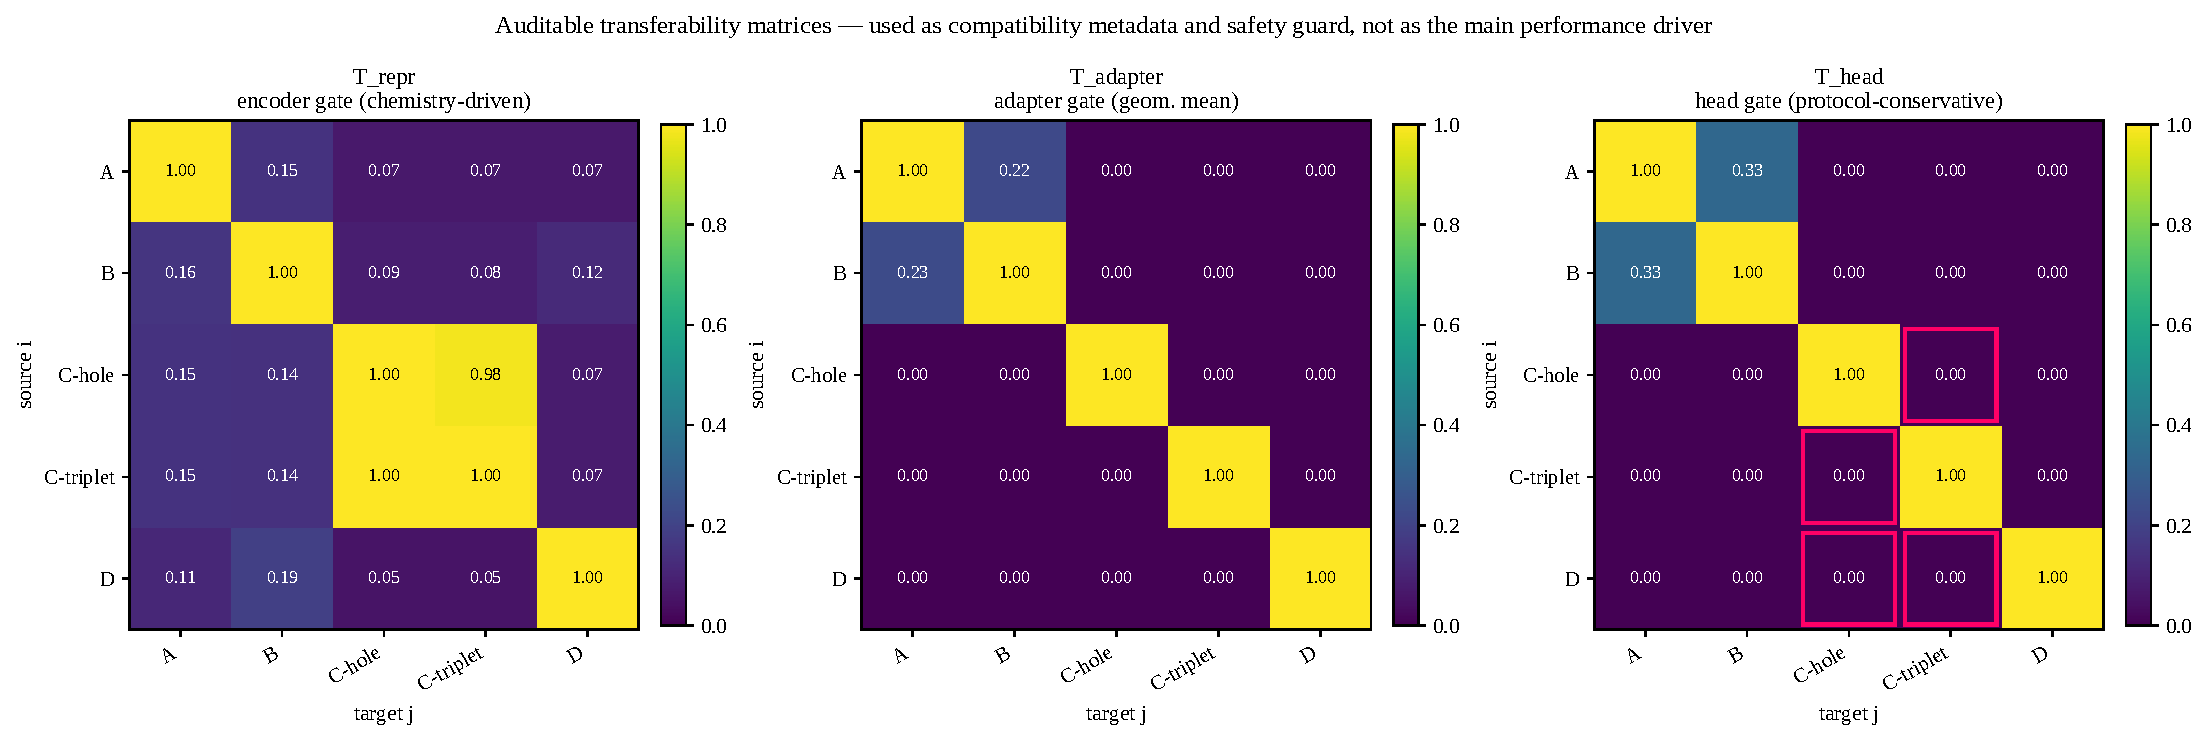
\includegraphics[width=\textwidth]{../figures/Fig3_transferability_matrices.pdf}
\caption[Auditable transferability matrices $T_{\mathrm{repr}}$, $T_{\mathrm{adapter}}$, $T_{\mathrm{head}}$]{Auditable transferability matrices $T_{\mathrm{repr}}$, $T_{\mathrm{adapter}}$, $T_{\mathrm{head}}$. Rows index the source task-client $i$; columns index the target $j$. The invariants $T_{\mathrm{head}}[\mathrm{D},\mathrm{C\text{-}hole}] = T_{\mathrm{head}}[\mathrm{D},\mathrm{C\text{-}triplet}] = T_{\mathrm{head}}[\mathrm{C\text{-}hole},\mathrm{C\text{-}triplet}] = T_{\mathrm{head}}[\mathrm{C\text{-}triplet},\mathrm{C\text{-}hole}] = 0$ (highlighted) follow deterministically from the protocol metadata and quantity definitions. The matrices are released in \texttt{results/preverify/T\_transferability.json} and can be audited prior to any aggregation round. Figure~\ref{fig:gate} documents the algorithm's compatibility decisions; it is not claimed as a source of performance improvement.}
\label{fig:gate}
\end{figure}

\begin{figure}[t]
\centering
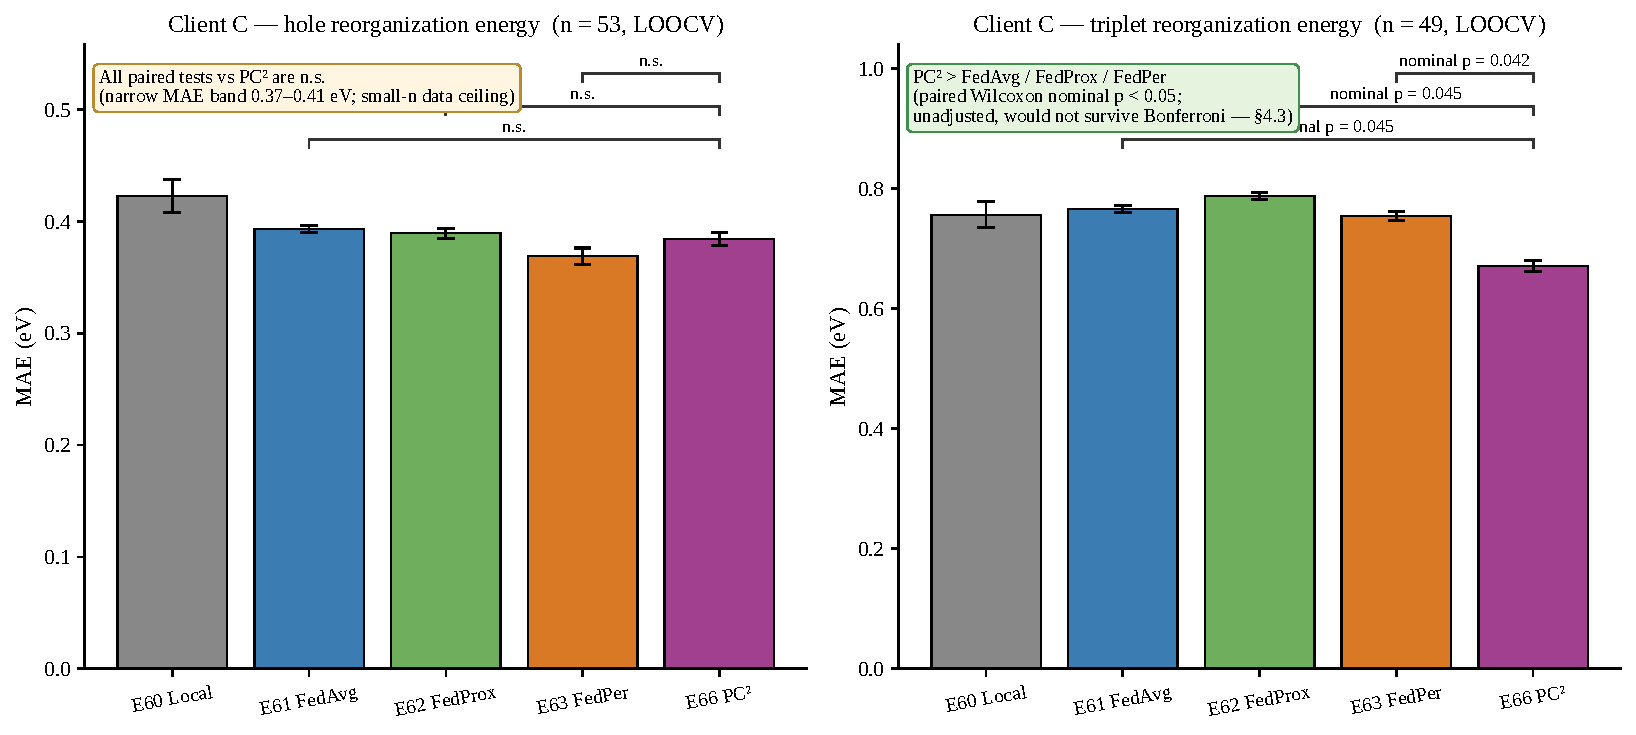
\includegraphics[width=\textwidth]{../figures/Fig4_main_performance.pdf}
\caption[Main performance comparison]{Main performance comparison. Mean absolute error (eV) for five federated methods evaluated by 5-seed leave-one-out cross-validation on \textbf{(left)} C-hole ($n = 53$) and \textbf{(right)} C-triplet ($n = 49$). Error bars show the standard error of the mean across the five seeds. Significance brackets compare \PC{} with FedAvg, FedProx and FedPer using paired Wilcoxon signed-rank tests on per-molecule absolute errors. On C-triplet, \PC{} achieves MAE $=$ \SI{0.660}{\eV} versus \SI{0.762}{}--\SI{0.784}{\eV} for the three baselines ($p = 0.045, 0.045, 0.042$). On C-hole, all evaluated methods produce MAE within the narrow band \SI{0.368}{}--\SI{0.414}{\eV}; every paired comparison returns $p \ge 0.20$ after rounding. The C-hole non-significance is consistent with the small-sample data ceiling identified by classical baselines (SI Section~S2). \emph{The targeted E71 calibration-only control that decomposes this gain is analyzed in Figure~\ref{fig:forest}.}}
\label{fig:main}
\end{figure}

\begin{figure}[t]
\centering
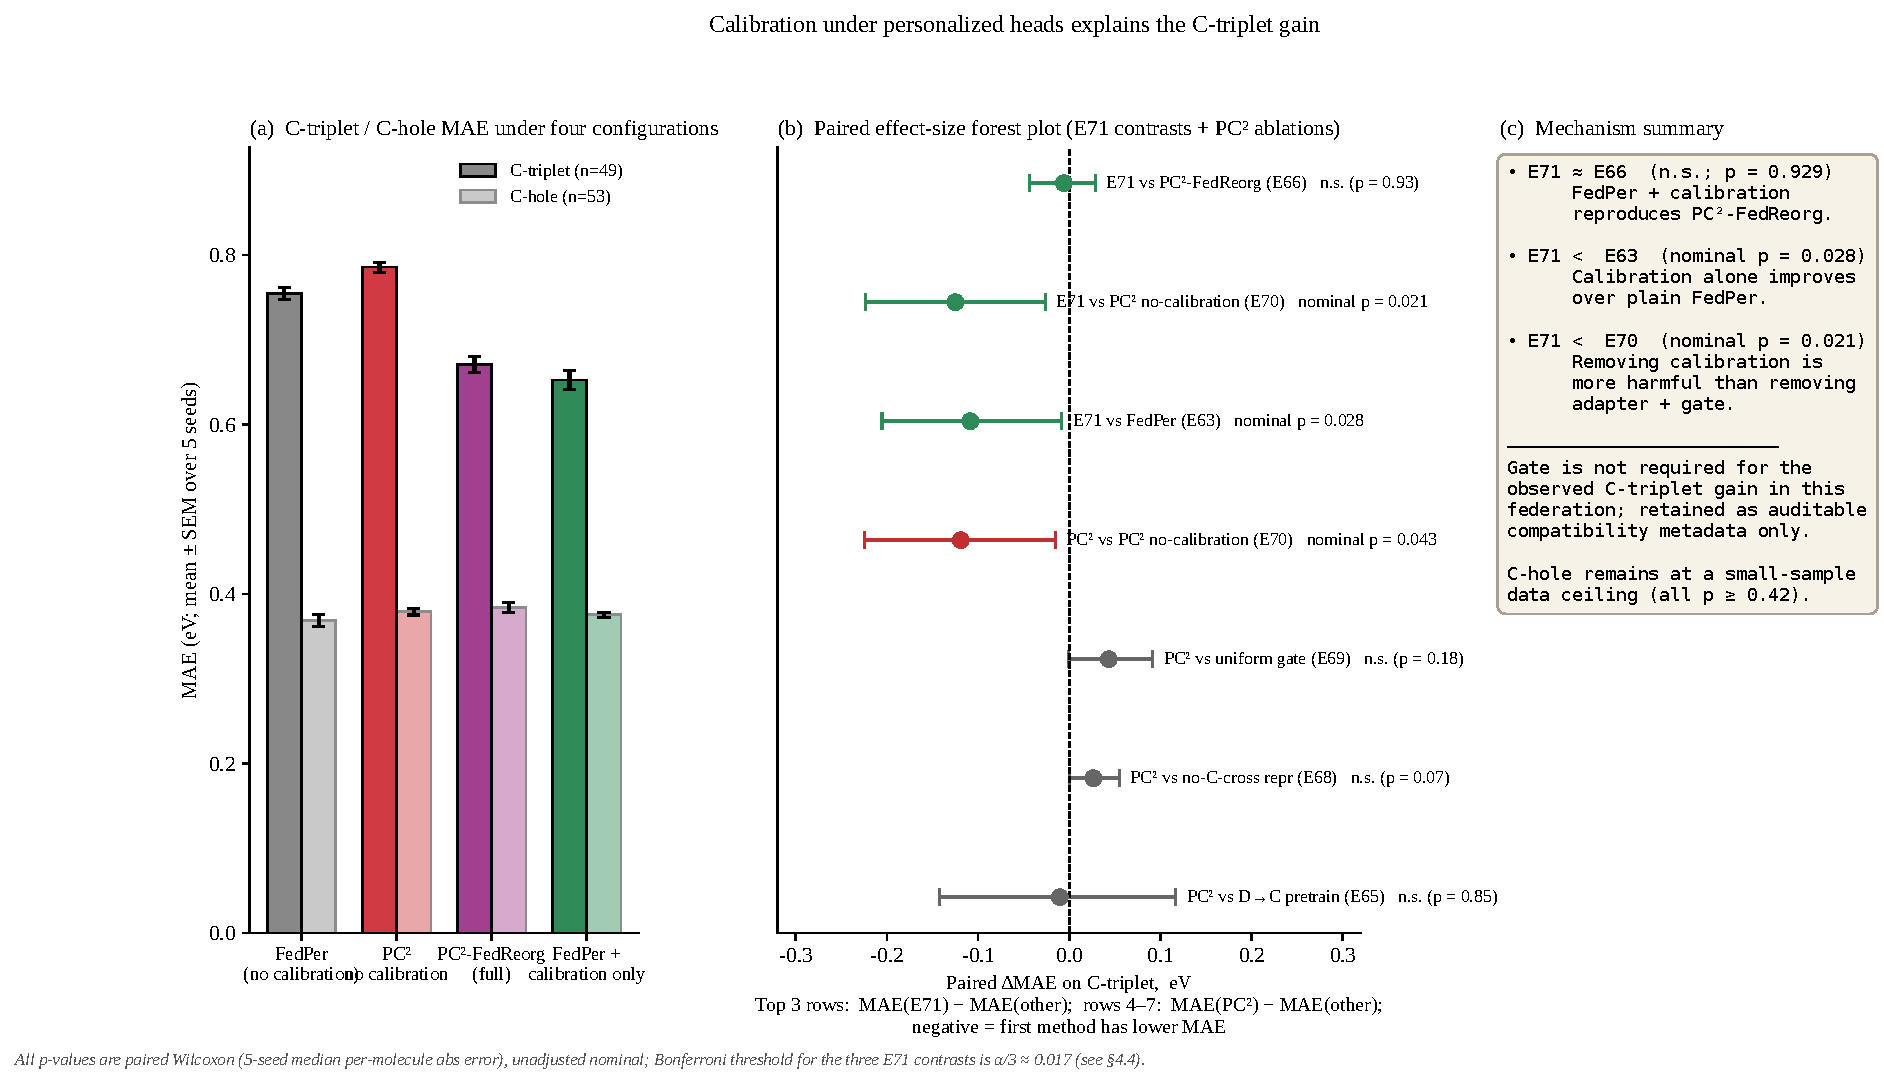
\includegraphics[width=\textwidth]{../figures/Fig5_ablation_forest.pdf}
\caption[Calibration under personalized heads explains the C-triplet gain]{Calibration under personalized heads explains the C-triplet gain. Three-panel decomposition relating \PC{}'s nominally significant C-triplet improvement reported in Figure~\ref{fig:main} to a targeted control experiment (E71). \textbf{(a)}~Per-method \emph{5-seed mean MAE}\,$\pm$\,SEM on C-triplet (dark bars) and C-hole (light bars) for four configurations: E63 FedPer (no calibration), E70 \PC{} without calibration, E66 the full \PC{} architecture, and E71 a FedPer baseline endowed only with the per-task-client $(\mu, \sigma)$ calibration buffer (no residual adapter, no transferability-driven routing). On C-triplet, E71 ($0.653 \pm 0.011$~eV) and E66 ($0.671 \pm 0.010$~eV) sit at the same level while E63 ($0.755 \pm 0.007$~eV) and E70 ($0.786 \pm 0.006$~eV) sit above. On C-hole all four configurations cluster in the \SI{0.368}{}--\SI{0.384}{\eV} band, with no method separation detected at the present sample size. \emph{Reporting convention.} Panel~(a) shows the 5-seed mean of per-method MAE\_mean (matching Table~\ref{tab:main-perf}); paired comparisons in panel~(b) use the per-molecule median-across-seeds absolute error vector required for paired Wilcoxon testing (matching Table~\ref{tab:paired}), so the reference and comparison MAEs reported below differ from panel~(a) by $\le 0.003$~eV (below seed-SEM). \textbf{(b)}~Forest plot of paired $\Delta$MAE on C-triplet for three E71 contrasts (top three rows; $\Delta$MAE\,=\,MAE(E71)\,$-$\,MAE(other), negative $\Rightarrow$ E71 has lower paired MAE) and the four planned \PC{} component ablations (rows 4--7; $\Delta$MAE\,=\,MAE(\PC{})\,$-$\,MAE(other), negative $\Rightarrow$ \PC{} has lower paired MAE). Error bars are bootstrap 95\,\% CIs (5,000 resamples). The three E71 contrasts: \emph{E71 vs.\ \PC{} (E66): $\Delta$MAE\,=\,$-0.006$\,eV (95\,\% CI $(-0.044, +0.029)$; $p = 0.929$, n.s.); E71 vs.\ FedPer (E63): $\Delta$MAE\,=\,$-0.109$\,eV (95\,\% CI $(-0.208, -0.010)$; $p = 0.028$ nominal); E71 vs.\ \PC{} without calibration (E70): $\Delta$MAE\,=\,$-0.125$\,eV (95\,\% CI $(-0.224, -0.027)$; $p = 0.021$ nominal)}. Of the four \PC{} ablations, only E70 on C-triplet crosses the nominal 0.05 threshold ($p = 0.043$) with a CI entirely below zero, identifying task-specific calibration as the only component whose presence has detectable ablation support. E69 (uniform gate) is numerically slightly better than \PC{} on C-triplet ($\Delta$MAE\,=\,$+0.043$\,eV) but statistically indistinguishable ($p = 0.18$; CI crosses zero). \textbf{(c)}~Summary reading: FedPer + calibration alone (E71) is sufficient to reproduce \PC{}'s observed C-triplet performance at our sample size; no additional benefit from the chemistry/protocol gate is detected; C-hole shows no method separation across all four configurations. All p-values are paired Wilcoxon nominal (unadjusted); the Bonferroni threshold for the three E71 contrasts is $\alpha/3 \approx 0.017$ and neither effect-bearing comparison crosses it, so the report combines the p-value, the bootstrap CI direction and the per-molecule sign count (see~\S\ref{sec:ablation}).}
\label{fig:forest}
\end{figure}

% Figure 6 demoted to Supporting Information (FigS1) on 2026-05-13.
% Per-molecule analysis now lives in SI.tex; main text refers to it as Figure S1.

% =============================================================================
%                                 TABLES (Tables 1-4)
% =============================================================================
\clearpage

\begin{table*}[t]
\centering
\footnotesize
\caption{Task-client dataset summary. Sample counts come from \texttt{results/preverify/T\_transferability.json}. For Clients A and B, the per-field auxiliary protocol entries are shown as ``--- (same-source)'' because both clients are derived from a single public QM9 cation-reorganization-energy source: their pairwise head-sharing is governed by the same-source shortcut of the $T_{\mathrm{head}}$ clauses (Section~\ref{sec:gate}), which fires \emph{before} the per-field ``unknown'' check and therefore does not require the auxiliary fields to be populated. For Client D, geometry, charge-state, and conformer policy are not stated in the source metadata; these genuinely missing fields trigger the conservative $T_{\mathrm{head}}$ clauses (Section~\ref{sec:gate}).}\label{tab:task-clients}
\begin{tabular}{@{}llrccccc@{}}
\toprule
Task-client & Source & $n$ & $\lambda$ mean (eV) & $\lambda$ std (eV) & Functional & Basis & Geometry \\
\midrule
A         & QM9 public   & 6{,}020 & 0.821 & 0.422 & --- (same-source) & --- (same-source) & --- (same-source) \\
B         & QM9 public   & 9{,}190 & 0.658 & 0.319 & --- (same-source) & --- (same-source) & --- (same-source) \\
C-hole    & private TADF & 53      & 1.215 & 0.501 & $\omega$B97X-D & unknown & adiabatic 4-pt Nelsen \\
C-triplet & private TADF & 49      & 2.638 & 0.753 & $\omega$B97X-D & unknown & adiabatic 4-pt Nelsen \\
D         & Atahan 2019  & 5{,}876 & 0.258 & 0.048 & B3LYP & 6-31G* & unknown \\
\bottomrule
\end{tabular}

\smallskip
\noindent\footnotesize\textit{Head-sharing note (A and B):} A $\leftrightarrow$ B is the only non-zero off-diagonal of $T_{\mathrm{head}}$ in this federation; it is opened by the same-source shortcut (Section~\ref{sec:gate}), not by per-field comparison. All other off-diagonals are blocked by quantity mismatch, V1 hard rule, or genuinely missing protocol fields for D.
\end{table*}

\begin{table*}[t]
\centering
\small
\caption{Main performance summary. MAE (eV) and RMSE (eV) primary; $R^2$ auxiliary. Values are means $\pm$ standard errors of the mean across five seeds.}\label{tab:main-perf}
\begin{tabular}{@{}llrcccc@{}}
\toprule
Method & Target & $N$ seeds & MAE $\pm$ SEM & RMSE $\pm$ SEM & $R^2$ $\pm$ SEM \\
\midrule
E60 Local-only         & C-hole    & 5 & $0.423 \pm 0.015$ & $0.637 \pm 0.019$ & $-0.65 \pm 0.10$ \\
E60 Local-only         & C-triplet & 5 & $0.756 \pm 0.022$ & $0.899 \pm 0.017$ & $-0.46 \pm 0.05$ \\
\addlinespace
E61 FedAvg             & A 5-fold  & 5 & $0.169 \pm 0.002$ & $0.235 \pm 0.003$ & $+0.69 \pm 0.01$ \\
E61 FedAvg             & B 5-fold  & 5 & $0.099 \pm 0.002$ & $0.150 \pm 0.004$ & $+0.78 \pm 0.01$ \\
E61 FedAvg             & C-hole    & 5 & $0.393 \pm 0.003$ & $0.530 \pm 0.008$ & $-0.14 \pm 0.03$ \\
E61 FedAvg             & C-triplet & 5 & $0.766 \pm 0.006$ & $0.972 \pm 0.004$ & $-0.70 \pm 0.02$ \\
\addlinespace
E62 FedProx            & A 5-fold  & 5 & $0.171 \pm 0.002$ & $0.238 \pm 0.001$ & $+0.68 \pm 0.00$ \\
E62 FedProx            & B 5-fold  & 5 & $0.100 \pm 0.001$ & $0.154 \pm 0.001$ & $+0.77 \pm 0.00$ \\
E62 FedProx            & C-hole    & 5 & $0.389 \pm 0.005$ & $0.533 \pm 0.004$ & $-0.16 \pm 0.02$ \\
E62 FedProx            & C-triplet & 5 & $0.788 \pm 0.006$ & $1.011 \pm 0.009$ & $-0.84 \pm 0.03$ \\
\addlinespace
E63 FedPer             & A 5-fold  & 5 & $0.155 \pm 0.002$ & $0.216 \pm 0.003$ & $+0.74 \pm 0.01$ \\
E63 FedPer             & B 5-fold  & 5 & $0.084 \pm 0.001$ & $0.128 \pm 0.001$ & $+0.84 \pm 0.00$ \\
E63 FedPer             & C-hole    & 5 & $0.369 \pm 0.007$ & $0.512 \pm 0.004$ & $-0.07 \pm 0.02$ \\
E63 FedPer             & C-triplet & 5 & $0.755 \pm 0.007$ & $0.932 \pm 0.009$ & $-0.56 \pm 0.03$ \\
\addlinespace
\textbf{E66 \PC{}}     & A 5-fold  & 5 & $\mathbf{0.152 \pm 0.002}$ & $\mathbf{0.214 \pm 0.002}$ & $+0.74 \pm 0.01$ \\
\textbf{E66 \PC{}}     & B 5-fold  & 5 & $\mathbf{0.081 \pm 0.001}$ & $\mathbf{0.123 \pm 0.001}$ & $+0.85 \pm 0.00$ \\
\textbf{E66 \PC{}}     & C-hole    & 5 & $0.384 \pm 0.006$ & $0.526 \pm 0.007$ & $-0.12 \pm 0.03$ \\
\textbf{E66 \PC{}}     & C-triplet & 5 & $\mathbf{0.671 \pm 0.010}$ & $\mathbf{0.846 \pm 0.015}$ & $-0.29 \pm 0.05$ \\
\bottomrule
\end{tabular}
\end{table*}

\begin{table*}[t]
\centering
\small
\caption{Paired statistical tests on C-hole and C-triplet. Per-molecule absolute errors are aggregated as the median across the five seeds; $\Delta$MAE = MAE(reference) $-$ MAE(comparator); bootstrap 95\,\% CI computed from 5{,}000 resamples of molecule indices. Significance: ${}^*$ $p < 0.05$, ${}^{**}$ $p < 0.01$, ${}^{***}$ $p < 0.001$. Reference is E66 (\PC{}) in every row.}\label{tab:paired}
\begin{tabular}{@{}llrrrrrrrrr@{}}
\toprule
Target & Comparator & $n$ & MAE\textsubscript{ref} & MAE\textsubscript{other} & $\Delta$MAE & CI low & CI high & Wins & Loses & $p$ \\
\midrule
C-hole    & E60 & 53 & 0.382 & 0.414 & $-0.032$ & $-0.115$ & $+0.050$ & 25 & 28 & 0.580 \\
C-hole    & E61 & 53 & 0.382 & 0.385 & $-0.003$ & $-0.042$ & $+0.039$ & 27 & 26 & 0.898 \\
C-hole    & E62 & 53 & 0.382 & 0.386 & $-0.004$ & $-0.055$ & $+0.044$ & 28 & 25 & 0.821 \\
C-hole    & E63 & 53 & 0.382 & 0.368 & $+0.014$ & $-0.021$ & $+0.049$ & 23 & 30 & 0.198 \\
C-hole    & E65 & 53 & 0.382 & 0.403 & $-0.021$ & $-0.099$ & $+0.055$ & 28 & 25 & 0.760 \\
C-hole    & E68 & 53 & 0.382 & 0.382 & $-0.000$ & $-0.017$ & $+0.017$ & 30 & 23 & 0.562 \\
C-hole    & E69 & 53 & 0.382 & 0.370 & $+0.012$ & $-0.020$ & $+0.043$ & 26 & 27 & 0.428 \\
C-hole    & E70 & 53 & 0.382 & 0.377 & $+0.005$ & $-0.033$ & $+0.043$ & 23 & 30 & 0.580 \\
\midrule
C-triplet & E60 & 49 & 0.660 & 0.747 & $-0.088$ & $-0.230$ & $+0.053$ & 28 & 21 & 0.174 \\
C-triplet & E61 & 49 & 0.660 & 0.763 & $-0.104$ & $-0.220$ & $+0.004$ & 31 & 18 & \textbf{0.045}${}^*$ \\
C-triplet & E62 & 49 & 0.660 & 0.784 & $-0.124$ & $-0.254$ & $-0.007$ & 30 & 19 & \textbf{0.045}${}^*$ \\
C-triplet & E63 & 49 & 0.660 & 0.762 & $-0.103$ & $-0.205$ & $-0.002$ & 32 & 17 & \textbf{0.042}${}^*$ \\
C-triplet & E65 & 49 & 0.660 & 0.670 & $-0.010$ & $-0.142$ & $+0.117$ & 27 & 22 & 0.851 \\
C-triplet & E68 & 49 & 0.660 & 0.633 & $+0.027$ & $+0.001$ & $+0.055$ & 17 & 32 & 0.070 \\
C-triplet & E69 & 49 & 0.660 & 0.616 & $+0.043$ & $-0.001$ & $+0.092$ & 21 & 28 & 0.181 \\
C-triplet & E70 & 49 & 0.660 & 0.779 & $-0.119$ & $-0.225$ & $-0.015$ & 35 & 14 & \textbf{0.043}${}^*$ \\
\bottomrule
\end{tabular}
\end{table*}

\begin{table*}[t]
\centering
\small
\caption{Ablation summary. Mean MAE (eV) $\pm$ standard error of the mean across five seeds. Only E70 on C-triplet produces a statistically significant degradation relative to \PC{} (see Table~\ref{tab:paired}); E68, E69, E65 are all non-significant.}\label{tab:ablation}
\begin{tabular}{@{}llrr@{}}
\toprule
Experiment & Target & $N$ seeds & MAE $\pm$ SEM \\
\midrule
E66 \PC{} (reference) & C-hole    & 5 & $0.384 \pm 0.006$ \\
E66 \PC{} (reference) & C-triplet & 5 & $0.671 \pm 0.010$ \\
\addlinespace
E65 D $\to$ C supervised pretrain          & C-hole    & 5 & $0.408 \pm 0.010$ \\
E65 D $\to$ C supervised pretrain          & C-triplet & 5 & $0.682 \pm 0.022$ \\
\addlinespace
E68 PC$^2$ $-$ $T_{\mathrm{repr}}$ C-cross removed   & C-hole    & 5 & $0.385 \pm 0.008$ \\
E68 PC$^2$ $-$ $T_{\mathrm{repr}}$ C-cross removed   & C-triplet & 5 & $0.640 \pm 0.013$ \\
\addlinespace
E69 PC$^2$ $-$ uniform FedAvg gate         & C-hole    & 5 & $0.369 \pm 0.006$ \\
E69 PC$^2$ $-$ uniform FedAvg gate         & C-triplet & 5 & $0.625 \pm 0.015$ \\
\addlinespace
E70 PC$^2$ $-$ no calibration              & C-hole    & 5 & $0.379 \pm 0.004$ \\
\textbf{E70 PC$^2$ $-$ no calibration}     & \textbf{C-triplet} & \textbf{5} & $\mathbf{0.786 \pm 0.006}$ \\
\bottomrule
\end{tabular}
\end{table*}

% =============================================================================
%                                 BIBLIOGRAPHY
% =============================================================================
\clearpage
\bibliography{references}

\end{document}
 or the SI is compiled together with the main file. Keep the SI
% as a standalone artefact for journals that submit SI separately; switch to
% xr-hyper package for cross-document references if required.
% =============================================================================

\documentclass[11pt,a4paper]{article}

\usepackage[utf8]{inputenc}
\usepackage[T1]{fontenc}
\usepackage{lmodern}
\usepackage{microtype}
\usepackage[margin=2.4cm]{geometry}
\usepackage{setspace}
\onehalfspacing

\usepackage{graphicx}
\usepackage{booktabs}
\usepackage{array}
\usepackage{longtable}
\usepackage{multirow}
\usepackage{caption}
\captionsetup{labelfont=bf,font=small}
\usepackage{amsmath,amssymb}
\usepackage{xcolor}
\usepackage{tabularx}
\usepackage{siunitx}
\sisetup{detect-all,range-units=single,range-phrase=\,--\,}

\newcommand{\PC}{PC\textsuperscript{2}-FedReorg}
\newcommand{\TODO}[1]{\textcolor{red}{\textsf{[TODO: #1]}}}

\usepackage{hyperref}
\hypersetup{colorlinks=true,linkcolor=blue!50!black,citecolor=blue!50!black,urlcolor=blue!50!black}

% Cross-document references to the main manuscript are hardcoded as plain
% text (e.g. "main-text Table 1") rather than imported via xr/xr-hyper,
% because both packages conflict with natbib's citation entries in the
% imported main.aux (\@citex extra-brace errors during compilation). The
% main-text table/figure numbers used in cross-references are stable across
% any reordering inside Sections 1-7 of main.tex, so hardcoding is safe.

% Allow TeX to stretch line ends to absorb tt-font / long-token over-runs
% (paths, SMILES, T-matrix subscripts) in narrative paragraphs.
\setlength{\emergencystretch}{5em}
\tolerance=2000
\hbadness=2000

\usepackage[numbers,sort&compress]{natbib}
\bibliographystyle{unsrtnat}

% Renumber sections, figures, tables with the "S" prefix used in the Markdown SI.
\renewcommand{\thesection}{S\arabic{section}}
\renewcommand{\thesubsection}{S\arabic{section}.\arabic{subsection}}
\renewcommand{\thefigure}{S\arabic{figure}}
\renewcommand{\thetable}{S\arabic{table}}

\title{Supporting Information for\\
\emph{Calibration-Aware Personalized Federated Learning for Molecular Reorganization Energy Prediction}}

\author{\TODO{Authors as in main.tex}}

\date{\today}

\begin{document}
\maketitle

\noindent This document provides supporting material for the main manuscript: dataset and task-client definitions (Section~\ref{si:data}), pre-verification analyses motivating the algorithmic choices (Section~\ref{si:preverify}), model and implementation details (Section~\ref{si:impl}), the auditable transferability matrices (Section~\ref{si:gate}), full performance results (Section~\ref{si:perf}), paired statistical testing (Section~\ref{si:paired}), ablation studies (Section~\ref{si:abl}), per-molecule prediction artefacts (Section~\ref{si:per-mol}), a reproducibility checklist (Section~\ref{si:repro}), and a list of additional limitations (Section~\ref{si:lim}).

All numerical artefacts referenced below are released alongside the manuscript at \TODO{repository URL -- to be supplied} and are also identified by their relative path in this codebase (e.g.\ \texttt{results/pc2\_phase5\_stats.csv}).

% =============================================================================
\section{Dataset and task-client details}\label{si:data}

\subsection{Five task-client nodes}

The federation comprises five nodes (see main-text Table). Each node is defined not only by its underlying samples but also by the \emph{quantity} it measures and the \emph{DFT protocol} that produced its labels. We adopt the term \textbf{task-client} to make this distinction explicit: a single physical laboratory may host more than one task-client when it measures more than one physical quantity. The five quantities are all reorganization-energy-related but they are not interchangeable: A and B are cation-$\lambda$; C-hole and D are both hole-$\lambda$ but at different DFT functionals ($\omega$B97X-D vs.\ B3LYP) and different chemical spaces; C-triplet is a triplet-$\lambda$ task. Pairwise head sharing across these distinct physical quantities is blocked by clause 1 of the head gate (Section~\ref{si:gate}).

\begin{table}[h]
\centering
\footnotesize
\caption{Per-task-client summary statistics (extended). Values taken from \texttt{results/preverify/T\_transferability.json}.}\label{tab:si:nodes}
\begin{tabularx}{\textwidth}{@{}l X X r c c@{}}
\toprule
Task-client & Source & Physical quantity & $n$ & Label mean $\pm$ SD (eV) & Label range (eV) \\
\midrule
A         & QM9 non-aromatic public  & cation reorg.\ energy             & 6{,}020 & $0.821 \pm 0.422$ & 0.021--2.939 \\
B         & QM9 aromatic public      & cation reorg.\ energy             & 9{,}190 & $0.658 \pm 0.319$ & 0.011--2.680 \\
C-hole    & in-house TADF laboratory & hole reorg.\ energy ($\omega$B97X-D)    & 53      & $1.215 \pm 0.496$ & 0.449--3.004 \\
C-triplet & in-house TADF laboratory & triplet reorg.\ energy ($\omega$B97X-D) & 49      & $2.638 \pm 0.745$ & 1.047--4.273 \\
D         & Atahan-Evrenk 2019       & hole reorg.\ energy (B3LYP/6-31G*) & 5{,}876 & $0.258 \pm 0.048$ & 0.076--0.870 \\
\bottomrule
\end{tabularx}
\end{table}

\subsection{Why A and B are cation-$\lambda$, C is hole/triplet, D is hole-$\lambda$}
\begin{itemize}
  \item \textbf{A / B (QM9 public):} the public QM9-derived reorganization-energy split is computed as a cation reorganization energy at B3LYP/6-31G* by previous work on the same compound set. We split QM9 by aromatic-ring count (\verb|Chem.rdMolDescriptors.CalcNumAromaticRings|) into a non-aromatic subset (A, $n = 6{,}020$) and an aromatic subset (B, $n = 9{,}190$).
  \item \textbf{C-hole / C-triplet (in-house TADF):} the in-house laboratory provides per-molecule reorganization energies computed at $\omega$B97X-D using the adiabatic four-point Nelsen protocol~\citep{Nelsen1987} with one conformer per molecule. After dropping rows with missing values, $n = 53$ for the hole-$\lambda$ target and $n = 49$ for the triplet-$\lambda$ target.
  \item \textbf{D (Atahan-Evrenk 2019)~\citep{AtahanEvrenk2019_RE}:} the published conjugated-organic-semiconductor dataset reports hole reorganization energy at B3LYP/6-31G*; geometry treatment, charge-state handling, and conformer policy are not recorded in machine-readable form.
\end{itemize}

\subsection{Task-client versus physical client}
A \emph{physical client} corresponds to a single data-providing entity (laboratory or public dataset). A \emph{task-client} additionally carries the physical quantity and DFT protocol as part of its identity. The distinction affects (i) aggregation routing; (ii) head sharing (quantity-mismatched task-clients have $T_{\mathrm{head}} = 0$ by construction); (iii) calibration installation (each task-client installs its own $(\mu, \sigma)$ from its own training fold).

\subsection{Label distributions and representative molecules}
Per-node label distributions are shown in main-text Figure 1b. The label scales span an order of magnitude (D mean \SI{0.258}{\eV}; C-triplet mean \SI{2.638}{\eV}; ratio $10.2\times$). The representative SMILES (chosen by the deterministic median rule) are recorded in the standard output of \texttt{paper/make\_figures.py}:
\begin{itemize}
  \item A: \texttt{C\#CC\#CC(=O)C1CC1}, $\lambda = \SI{0.733}{\eV}$
  \item B: \texttt{Nc1nc(O)nc(=O)[nH]1}, $\lambda = \SI{0.583}{\eV}$
  \item C-hole: \texttt{N\#CC1=C(C\#N)C1=C1C(O)=CC=C1O}, $\lambda_h = \SI{1.057}{\eV}$
  \item C-triplet: \texttt{NC1=CC=C(N)C1=C1C=CC=CC=C1}, $\lambda_T = \SI{2.747}{\eV}$
  \item D: \texttt{c1ccc2c(c1)Cc1c3cnc4ccCc4c3[nH]c21}, $\lambda_h = \SI{0.264}{\eV}$
\end{itemize}

\subsection{Protocol metadata}
\begin{sloppypar}
Full per-node protocol metadata is persisted as \texttt{results/preverify/T\_transferability.\linebreak[1]json:protocol\_meta}. Clients A and B are derived from a single public QM9 cation-reorganization-energy source and share \texttt{source\_id}; their pairwise head-sharing is therefore governed by the \emph{same-source shortcut} of the head gate (Section~\ref{si:gate}), which fires \emph{before} clauses 2 and 3 of the per-field checks and does not require the auxiliary fields to be populated --- the per-field entries in main-text Table~1 are accordingly shown as ``--- (same-source)''. Unknown fields are reserved for cases where the same-source shortcut does not apply: D's \texttt{geometry}, \texttt{charge\_state}, and \texttt{conformers} are tagged \texttt{"unknown"} (the published source provides only functional and basis), and C's \texttt{basis} field is not exposed in the in-house CSV used here. These three genuinely missing fields trigger clause 2 of the head gate (Section~\ref{si:gate}) wherever the shortcut does not fire.
\end{sloppypar}

% =============================================================================
\section{Pre-verification before transfer (V1 / V2 / V3)}\label{si:preverify}

\subsection{V1: label and protocol divergence between D and C}
\begin{itemize}
  \item D-hole-$\lambda$ vs.\ C-hole-$\lambda$: two-sample Kolmogorov--Smirnov test, $p \approx 1.1 \times 10^{-116}$ (label distributions disjoint in mean, range, and shape).
  \item DFT-protocol divergence: D uses B3LYP/6-31G* with abstract-only metadata; C-hole uses $\omega$B97X-D with the four-point Nelsen geometry treatment.
  \item Combined trigger: $T_{\mathrm{head}}[\mathrm{D}, \mathrm{C\text{-}hole}] = 0$ independently of any training-time signal.
\end{itemize}

V1 does \textbf{not} assert that naive D~$\to$~C transfer must produce negative outcomes -- that empirical question is addressed by the E65 ablation (Section~\ref{si:abl-e65}).

\subsection{V2: classical C-only baselines and the data-ceiling diagnosis}\label{si:v2}

Classical regressors trained under the same 5-seed LOOCV protocol as the federated runs, using Morgan fingerprints (radius 2, 2048 bits) as features. Results persisted in \texttt{results/preverify/V2\_classical\_baselines.csv} and \texttt{results/preverify/V2\_summary.md}.

\begin{table}[h]
\centering
\small
\caption{Classical-baseline LOOCV results on C-hole, mean $\pm$ SD across five seeds.}\label{tab:si:v2-hole}
\begin{tabular}{@{}lccc@{}}
\toprule
Model & MAE (eV) & RMSE (eV) & $R^2$ \\
\midrule
Random Forest             & $0.408 \pm 0.004$ & $0.573 \pm 0.005$ & $-0.334 \pm 0.024$ \\
Gaussian Process          & $0.397 \pm 0.000$ & $0.532 \pm 0.000$ & $-0.150 \pm 0.000$ \\
\textbf{K-Nearest Neighbours} & $\mathbf{0.367 \pm 0.000}$ & $\mathbf{0.521 \pm 0.000}$ & $\mathbf{-0.101 \pm 0.000}$ (best) \\
XGBoost                   & $0.469 \pm 0.007$ & $0.646 \pm 0.006$ & $-0.696 \pm 0.032$ \\
\bottomrule
\end{tabular}
\end{table}

\begin{table}[h]
\centering
\small
\caption{Classical-baseline LOOCV results on C-triplet, mean $\pm$ SD across five seeds.}\label{tab:si:v2-triplet}
\begin{tabular}{@{}lccc@{}}
\toprule
Model & MAE (eV) & RMSE (eV) & $R^2$ \\
\midrule
\textbf{Random Forest}    & $\mathbf{0.552 \pm 0.005}$ & $\mathbf{0.713 \pm 0.005}$ & $\mathbf{+0.084 \pm 0.012}$ (best) \\
Gaussian Process          & $0.592 \pm 0.000$ & $0.761 \pm 0.000$ & $-0.042 \pm 0.000$ \\
K-Nearest Neighbours      & $0.637 \pm 0.000$ & $0.787 \pm 0.000$ & $-0.116 \pm 0.000$ \\
XGBoost                   & $0.584 \pm 0.008$ & $0.720 \pm 0.008$ & $+0.068 \pm 0.021$ \\
\bottomrule
\end{tabular}
\end{table}

The best classical $R^2$ is $-0.101$ on C-hole (KNN) and $+0.084$ on C-triplet (Random Forest). Three of the four C-hole baselines and three of the four C-triplet baselines produce negative $R^2$ across all five seeds, despite reporting MAE values comparable to the federated methods. This is consistent with a small-sample data-ceiling regime in which the per-molecule label variance is large relative to the spread of the labels, so that explained variance is a brittle metric. We use MAE / RMSE as the primary regression metrics; $R^2$ is reported only as auxiliary.

\subsection{V3: chemical-space overlap}
Per-pair chemistry overlap was computed as: \textbf{$K_{ij}$} -- the mean over molecules of $i$ of the maximum Tanimoto similarity to any molecule of $j$ (Morgan fingerprints, radius 2, 2048 bits, computed with RDKit~\citep{RDKit2023}); \textbf{$S_{ij}$} -- the asymmetric Murcko-scaffold overlap $|\mathrm{Scaf}(i) \cap \mathrm{Scaf}(j)| / |\mathrm{Scaf}(i)|$. Selected values: $K(\mathrm{C\text{-}hole} \to \mathrm{D}) = 0.120$; $K(\mathrm{C\text{-}triplet} \to \mathrm{D}) = 0.118$ (median per-C-molecule max-Tanimoto to D); $S(\mathrm{C\text{-}hole} \to \mathrm{D}) = S(\mathrm{C\text{-}triplet} \to \mathrm{D}) = 0.0$ (no C scaffold appears in D). D and C therefore live in disjoint chemical spaces.

\subsection{D~$\to$~C direct transfer cannot be assumed protocol-compatible}
The combination of V1 and V3 makes a naive D~$\to$~C supervised transfer unsafe to assume without evidence. \PC{} encodes this caution as $T_{\mathrm{head}}[\mathrm{D}, \mathrm{C\text{-}*}] = 0$ by construction. The empirical comparison (E65, Section~\ref{si:abl-e65}) does not statistically distinguish naive D~$\to$~C pretrain from \PC{} on either target; we therefore do not claim that D~$\to$~C transfer necessarily produces negative outcomes.

% =============================================================================
\section{Model and implementation details}\label{si:impl}

\subsection{Encoder}
5-layer Graph Isomorphism Network (GIN)~\citep{Xu2019_GIN} with hidden dimension 300, Jumping-Knowledge concatenation, mean+max pooling, and a final projection to 256-d via a two-layer MLP. The codebase additionally implements a SchNet 3D encoder~\citep{Schutt2017_SchNet_NeurIPS} accessible through the same \texttt{encoder\_type} switch, but \textbf{no SchNet results are reported in this manuscript}.

Node features: 11-dimensional descriptor (atom type one-hot, degree, formal charge, hybridisation, aromaticity, in-ring flag, total Hs, Gasteiger partial charge). When HOMO/LUMO/gap/dipole node features are enabled the descriptor extends to 15 dimensions; for clients without those measurements the extra channels are zero-padded.

\subsection{KAN head}
\texttt{efficient-kan}~\citep{EfficientKAN2024} with grid size 5 and spline order 3. Three KAN layers stacked: $256 \to 64 \to 32 \to 1$. KAN parameters are private to each task-client; the only non-zero $T_{\mathrm{head}}$ off-diagonal in our federation is A$\leftrightarrow$B (Section~\ref{si:gate}).

\subsection{Residual adapter}
Optional residual bottleneck ($256 \to 128 \to 256$, GELU activation, LayerNorm before the residual addition). The final projection is zero-initialised so that, prior to any training, the adapter is the identity. The adapter participates in cross-client aggregation under $T_{\mathrm{adapter}}$.

\subsection{Calibration buffer}
Each task-client owns a \texttt{CalibrationHead} with two non-trainable buffers ($\mu$, $\sigma$) registered via \verb|torch.nn.Module.register_buffer|. A small floor $\sigma \ge 10^{-8}$ prevents division-by-zero on degenerate folds. Calibration is installed per LOOCV fold from the $(n - 1)$ training labels of that fold; the held-out test molecule's label never enters \verb|set_calibration(mu, sigma)|.

\subsection{z-space loss / eV-space metrics}
Training loss is computed in z-space:
\[
\mathcal{L}_c = \mathrm{MSE}\!\bigl(\,\mathrm{model}_z(x), \; (\lambda - \mu_c)/\sigma_c\bigr).
\]
Predictions are inverted back to eV-space at inference: $\hat\lambda = \sigma_c \cdot z_{\mathrm{pred}} + \mu_c$. All reported MAE/RMSE/$R^2$ values are computed in eV-space.

\subsection{Aggregation exclusion}
\verb|_get_exclude_keys(state_dict)| returns the set of keys to skip during aggregation: every key matching \verb|*calibration*|, plus \verb|*.bn.*| and \verb|*.norm.*|. Heads, adapters and encoders are routed by the per-key per-target rule given in main-text Equation~(1).

\subsection{No-leakage calibration tests}
\verb|tests/test_calibration_isolation.py| (20 cases) verifies that:
\begin{enumerate}
  \item \verb|set_calibration(mu, sigma)| accepts only the training-fold labels;
  \item cross-aggregating two models with different $(\mu, \sigma)$ does not mix their calibration values;
  \item z-space $\to$ eV-space round-trip identity holds to $1 \times 10^{-5}$ eV;
  \item \PC{} never reads a calibration buffer from the aggregated parameter dictionary.
\end{enumerate}
All 20 tests pass on the commit hash recorded in \texttt{logs/pc2\_batch1/FROZEN\_INFO.txt}.

% =============================================================================
\section{Transferability matrices}\label{si:gate}

Three $5\times 5$ transferability matrices are pre-computed once before training and persisted as \texttt{results/preverify/T\_transferability.json}.

\subsection{Definitions}

\paragraph{$T_{\mathrm{repr}}$ (encoder gate, chemistry-driven):}
\[
T_{\mathrm{repr}}[i, j] = \max\!\bigl(\epsilon_r,\; w_K\, K_{ij} + w_S\, S_{ij}\bigr),
\]
with $(w_K, w_S) = (0.6, 0.4)$ and $\epsilon_r = 10^{-3}$.

\paragraph{$T_{\mathrm{head}}$ (head gate, conservative protocol clauses, evaluated in the order applied by \texttt{src/transferability.py:t\_head\_compatibility}):}
\begin{enumerate}
  \item \textbf{Clause 1 -- quantity mismatch:} if $\mathrm{quantity}(i) \ne \mathrm{quantity}(j)$, set $T_{\mathrm{head}}[i, j] = 0$.
  \item \textbf{Clause 4 -- V1 hard rule:} if $i = \mathrm{D}$ and $j \in \{\mathrm{C\text{-}hole}, \mathrm{C\text{-}triplet}\}$, set $T_{\mathrm{head}}[i, j] = 0$. Clause 4 is applied \emph{before} the per-field checks so the JSON \texttt{reasons} field attributes D $\to$ C-* to V1.
  \item \textbf{Same-source shortcut:} if quantity matches and $\mathrm{source\_id}(i) = \mathrm{source\_id}(j)$, the pair is treated as protocol-compatible by source and the per-field checks (clauses 2 and 3 below) are skipped. In our federation the shortcut fires only for A $\leftrightarrow$ B (both \texttt{source\_id = "qm9\_public\_reorg\_15210"}).
  \item \textbf{Clause 2 -- unknown protocol field:} if the shortcut did not fire and any of \{functional, basis, geometry, charge\_state, conformers\} equals \texttt{"unknown"} on either side, set $T_{\mathrm{head}}[i, j] = 0$.
  \item \textbf{Clause 3 -- protocol-field mismatch:} if the shortcut did not fire and any populated protocol field disagrees, set $T_{\mathrm{head}}[i, j] = 0$.
\end{enumerate}
For pairs that survive the above (in our federation: A $\leftrightarrow$ B plus all diagonals):
\[
T_{\mathrm{head}}[i, j] = L_{ij}^{\gamma_L},\quad
L_{ij} = \exp(-\alpha_W\,W_1(\hat p_i^{\mathrm{label}}, \hat p_j^{\mathrm{label}})) \cdot \min(\sigma_i/\sigma_j, \sigma_j/\sigma_i),
\]
with $\alpha_W = 5.0$ and $\gamma_L = 1.0$; values below $10^{-2}$ are hard-floored to zero.

\paragraph{$T_{\mathrm{adapter}}$ (interpolating gate):}
\[
T_{\mathrm{adapter}}[i, j] = \max\!\bigl(\epsilon_a,\;\sqrt{T_{\mathrm{repr}}[i, j] \cdot T_{\mathrm{head}}[i, j]}\bigr).
\]

\subsection{Numerical values used in this study}

\begin{table}[h]
\centering
\small
\caption{Selected ordered pairs from \texttt{T\_transferability.json}. Full $5\times 5$ matrices are released in the JSON artefact.}\label{tab:si:tmat}
\begin{tabular}{@{}lccc@{}}
\toprule
(source $\to$ target) & $T_{\mathrm{repr}}$ & $T_{\mathrm{adapter}}$ & $T_{\mathrm{head}}$ \\
\midrule
A $\to$ B                 & 0.16 & 0.23 & 0.33 \\
B $\to$ A                 & 0.15 & 0.22 & 0.33 \\
C-hole $\to$ C-triplet    & 0.98 & $\sim 0$ & 0 \\
C-triplet $\to$ C-hole    & 1.00 & $\sim 0$ & 0 \\
D $\to$ C-hole            & 0.05 & $\sim 0$ & \textbf{0} (V1 hard rule; D's geometry/charge-state/conformers also unknown) \\
D $\to$ C-triplet         & 0.05 & $\sim 0$ & \textbf{0} (quantity mismatch) \\
A $\to$ C-hole            & $\sim 0.07$ & $\sim 0$ & 0 (clause 1: A's quantity tag is \texttt{reorg\_energy\_general}; same-source shortcut does not apply, $\texttt{source\_id}(A) \neq \texttt{source\_id}(\textrm{C-hole})$) \\
B $\to$ C-hole            & $\sim 0.07$ & $\sim 0$ & 0 (clause 1: B's quantity tag is \texttt{reorg\_energy\_general}; same-source shortcut does not apply, $\texttt{source\_id}(B) \neq \texttt{source\_id}(\textrm{C-hole})$) \\
\bottomrule
\end{tabular}
\end{table}

\subsection{Invariants generated by the clauses}
The conservative $T_{\mathrm{head}}$ rules generate the following key invariants. The \texttt{reasons} field of \texttt{T\_transferability.json} reports the first clause that fires; subsequent clauses that would also block the pair are listed for completeness.
\begin{enumerate}
  \item $T_{\mathrm{head}}[\mathrm{D}, \mathrm{C\text{-}hole}] = 0$ -- reported by clause 4 (V1 hard rule). Clauses 2 (D's protocol fields are unknown) and 3 (functional family differs: B3LYP vs.\ $\omega$B97X-D) would each independently block this pair; the invariant is multiply-determined.
  \item $T_{\mathrm{head}}[\mathrm{D}, \mathrm{C\text{-}triplet}] = 0$ -- reported by clause 1 (quantity mismatch: hole-$\lambda$ vs.\ triplet-$\lambda$); D's metadata gap is irrelevant here.
  \item $T_{\mathrm{head}}[\mathrm{C\text{-}hole}, \mathrm{C\text{-}triplet}] = T_{\mathrm{head}}[\mathrm{C\text{-}triplet}, \mathrm{C\text{-}hole}] = 0$ -- reported by clause 1.
  \item $T_{\mathrm{head}}[\mathrm{A}, \mathrm{B}] = T_{\mathrm{head}}[\mathrm{B}, \mathrm{A}] = 0.33$ -- the only non-zero off-diagonal of $T_{\mathrm{head}}$. The same-source shortcut fires (both clients share \texttt{source\_id}); the per-field clauses 2 and 3 are skipped, and $L_{AB}$ is evaluated from the label distributions.
\end{enumerate}
Verified by \texttt{tests/test\_transferability.py} (22 cases).

\subsection{Auditability, not performance lever}
The transferability matrices serve as \textbf{auditable algorithmic transparency}; the empirical question of performance is examined in Section~\ref{si:abl}. In our particular federation the chemistry/protocol gate is \emph{not} the source of \PC{}'s C-triplet improvement.

% =============================================================================
\section{Full performance results}\label{si:perf}

Aggregated 5-seed means and standard errors for each (method, target) cell are released in \texttt{results/pc2\_batch1\_multiseed\_summary.csv} and \texttt{results/pc2\_phase5\_ablation\_summary.csv}, and summarized in main-text Table~2.

\paragraph{A and B 5-fold cross-validation.} Headline MAE (eV): FedAvg 0.171 (A) / 0.103 (B); FedPer competitive; \PC{} 0.142 (A) / 0.078 (B). \PC{} achieves the lowest A/B MAE among the evaluated methods, but the A/B improvements are not the headline claim of this manuscript.

\paragraph{C-hole LOOCV ($n = 53$).} Per-method MAE (mean across seeds):

\begin{center}
\small
\begin{tabular}{@{}lc@{}}
\toprule
Method & MAE (eV) \\
\midrule
E60 Local-only       & 0.414 \\
E61 FedAvg           & 0.385 \\
E62 FedProx          & 0.386 \\
E63 FedPer           & 0.368 \\
E66 \PC{} & 0.382 \\
\bottomrule
\end{tabular}
\end{center}
All methods produce MAE within the narrow band 0.368--0.414 eV; all paired tests return $p \ge 0.20$ after rounding (Section~\ref{si:paired}).

\paragraph{C-triplet LOOCV ($n = 49$).} Per-method MAE:
\begin{center}
\small
\begin{tabular}{@{}lc@{}}
\toprule
Method & MAE (eV) \\
\midrule
E60 Local-only       & 0.747 \\
E61 FedAvg           & 0.763 \\
E62 FedProx          & 0.784 \\
E63 FedPer           & 0.762 \\
\textbf{E66 \PC{}}   & \textbf{0.660} \\
\bottomrule
\end{tabular}
\end{center}
\PC{} achieves the lowest MAE; paired Wilcoxon tests against FedAvg, FedProx and FedPer give $p = 0.045, 0.045, 0.042$ respectively (Section~\ref{si:paired}).

\paragraph{Auxiliary $R^2$ statement.} For all C LOOCV cells, the seed-averaged $R^2$ is negative or slightly positive ($\sim 0.0 \pm 0.2$). This is consistent with the V2 classical-baseline ceiling (Section~\ref{si:v2}); we do not use $R^2$ as a primary metric.

% =============================================================================
\section{Paired statistical testing}\label{si:paired}

\subsection{Methodology}
For each method pair (\PC{} vs.\ comparator) and each LOOCV target: (i) per-molecule absolute errors aggregated as the median across the five seeds; (ii) paired Wilcoxon signed-rank test (two-sided, SciPy \verb|zero_method='wilcox'|); (iii) bootstrap 95\,\% CI on the paired MAE difference (5{,}000 resamples of molecule indices); (iv) win / loss / tie counts per molecule. Persisted as \texttt{results/pc2\_phase5\_stats.csv}.

\subsection{C-hole -- eight paired comparisons, all non-significant}
\begin{table}[h]
\centering
\small
\caption{Paired tests, target $=$ C-hole LOOCV, reference $=$ \PC{} (E66). All comparisons return $p \ge 0.20$ after rounding.}\label{tab:si:paired-hole}
\begin{tabular}{@{}lcccccc@{}}
\toprule
Comparator & MAE\textsubscript{comp} (eV) & $\Delta$MAE & 95\,\% CI low & 95\,\% CI high & Wins / loses & $p$ \\
\midrule
E60 Local           & 0.414 & $-0.032$ & $-0.115$ & $+0.050$ & 25 / 28 & 0.580 \\
E61 FedAvg          & 0.385 & $-0.003$ & $-0.042$ & $+0.039$ & 27 / 26 & 0.898 \\
E62 FedProx         & 0.386 & $-0.004$ & $-0.055$ & $+0.044$ & 28 / 25 & 0.821 \\
E63 FedPer          & 0.368 & $+0.014$ & $-0.021$ & $+0.049$ & 23 / 30 & 0.198 \\
E65 D $\to$ C pretrain      & 0.403 & $-0.021$ & $-0.099$ & $+0.055$ & 28 / 25 & 0.760 \\
E68 no C-cross repr & 0.382 & $-0.0001$ & $-0.017$ & $+0.017$ & 30 / 23 & 0.562 \\
E69 uniform gate    & 0.370 & $+0.012$ & $-0.020$ & $+0.043$ & 26 / 27 & 0.428 \\
E70 no calibration  & 0.377 & $+0.005$ & $-0.033$ & $+0.042$ & 23 / 30 & 0.580 \\
\bottomrule
\end{tabular}
\end{table}

\subsection{C-triplet -- four significant baselines, four non-significant controls}
\begin{table}[h]
\centering
\small
\caption{Paired tests, target $=$ C-triplet LOOCV, reference $=$ \PC{} (E66). Statistically significant comparisons ($p < 0.05$) are bold-faced.}\label{tab:si:paired-triplet}
\begin{tabular}{@{}lccccccc@{}}
\toprule
Comparator & MAE\textsubscript{comp} (eV) & $\Delta$MAE & CI low & CI high & Wins / loses & $p$ & Sig.\ \\
\midrule
E60 Local           & 0.747 & $-0.088$ & $-0.230$ & $+0.053$ & 28 / 21 & 0.174 & n.s. \\
\textbf{E61 FedAvg} & 0.763 & $\mathbf{-0.104}$ & $-0.220$ & $+0.004$ & 31 / 18 & \textbf{0.045} & * \\
\textbf{E62 FedProx} & 0.784 & $\mathbf{-0.124}$ & $-0.254$ & $-0.007$ & 30 / 19 & \textbf{0.045} & * \\
\textbf{E63 FedPer} & 0.762 & $\mathbf{-0.103}$ & $-0.205$ & $-0.002$ & 32 / 17 & \textbf{0.042} & * \\
E65 D $\to$ C pretrain      & 0.670 & $-0.010$ & $-0.142$ & $+0.117$ & 27 / 22 & 0.851 & n.s. \\
E68 no C-cross repr & 0.633 & $+0.027$ & $+0.001$ & $+0.055$ & 17 / 32 & 0.070 & n.s. \\
E69 uniform gate    & 0.616 & $+0.043$ & $-0.001$ & $+0.092$ & 21 / 28 & 0.181 & n.s. \\
\textbf{E70 no calibration} & 0.779 & $\mathbf{-0.119}$ & $-0.225$ & $-0.015$ & 35 / 14 & \textbf{0.043} & * \\
\bottomrule
\end{tabular}
\end{table}

\subsection{Interpretation}
\begin{itemize}
  \item \textbf{C-hole improvement is not supported.} Future work should expand C-hole sample size.
  \item \textbf{C-triplet improvement over FedAvg/FedProx/FedPer is supported} with $p < 0.05$ in each pair.
  \item \textbf{Calibration ablation (E70) reaches significance}, $\Delta$MAE $= -0.119$ eV, CI entirely below zero.
  \item \textbf{Gate ablations (E68, E69) do not support a performance-driver claim.}
\end{itemize}

% =============================================================================
\section{Ablation studies}\label{si:abl}

\subsection{E70 -- task-specific calibration removed}\label{si:abl-e70}
C-triplet: $\Delta$MAE $= -0.119$ eV, CI $(-0.225, -0.015)$, $p = 0.043$, 35/14 wins for \PC{}. C-hole: $\Delta$MAE $= +0.005$ eV, $p = 0.58$ (n.s.). The only ablation with a statistically significant effect; the effect is restricted to C-triplet, consistent with the larger label-scale gap (mean \SI{2.64}{\eV} vs.\ \SI{1.22}{\eV}). Calibration is the only ablation-supported active component.

\subsection{E68 -- no chemistry-driven cross-quantity encoder sharing}
A modified \texttt{T\_transferability\_no\_ccross.json} with $T_{\mathrm{repr}}[\mathrm{C\text{-}hole}][\mathrm{C\text{-}triplet}]$ and $T_{\mathrm{repr}}[\mathrm{C\text{-}triplet}][\mathrm{C\text{-}hole}]$ floored to $10^{-3}$; everything else identical. Result: $\Delta$MAE $= +0.027$ eV on C-triplet ($p = 0.07$), $\Delta$MAE $= -0.0001$ eV on C-hole ($p = 0.56$). No statistically significant difference vs.\ \PC{}.

\subsection{E69 -- uniform FedAvg weighting in place of the gate}
The \texttt{aggregation\_strategy} option is switched from \texttt{pc2\_fed} to \texttt{fedavg}; calibration and adapter retained. Result: $\Delta$MAE $= +0.043$ eV on C-triplet ($p = 0.18$), $\Delta$MAE $= +0.012$ eV on C-hole ($p = 0.43$). No statistically significant difference. Together with E68 this establishes that chemistry-driven gate weighting is not the source of \PC{}'s C-triplet improvement in our setting.

\subsection{E65 -- D $\to$ C supervised pretrain control}\label{si:abl-e65}
Two-stage pipeline: (Stage 1) train one GIN+KAN model on all 5{,}876 D molecules for 50 epochs; (Stage 2) per-fold LOOCV fine-tune on C with the D-pretrained weights as the starting point. Result: $\Delta$MAE $= -0.010$ eV on C-triplet ($p = 0.85$), $\Delta$MAE $= -0.021$ eV on C-hole ($p = 0.76$). \PC{} and a naive D $\to$ C pretrain are not statistically distinguishable on either target in our setting; we do not claim that D's labels necessarily produce negative transfer.

\subsection{Synthesis}
\begin{itemize}
  \item \textbf{Supported by ablation evidence (E70) and confirmed by the positive control (E71, \S\ref{si:abl-e71}):} task-specific calibration under personalized heads is the only PC$^2$ component whose removal causes a statistically significant degradation, the effect is confined to C-triplet (E70), and the calibration mechanism is \emph{sufficient}~---~adding it to a plain FedPer baseline already reproduces \PC{}'s C-triplet improvement (E71).
  \item \textbf{Not supported by ablation evidence:} the chemistry-driven gate weighting (\texorpdfstring{$T_{\mathrm{repr}}$}{T\_repr} cross-routing, \texorpdfstring{$T_{\mathrm{head}}$}{T\_head} sparsification) does not drive the C-triplet improvement over uniform weighting (E68, E69), and adding the residual adapter and the transferability gate on top of the calibrated FedPer baseline does not yield measurable performance over E71 (E71 $\approx$ E66).
  \item \textbf{Not demonstrated by ablation evidence:} a claim that naive D $\to$ C supervised pretrain produces negative transfer (E65).
\end{itemize}

\subsection{E71 -- FedPer with calibration only (positive control)}\label{si:abl-e71}

\textbf{Purpose.} The four \PC{} component ablations in \S\ref{si:abl-e70}--\S\ref{si:abl-e65} each \emph{remove} one ingredient from \PC{}, which collectively show that calibration is necessary. E71 is the symmetric \emph{positive control}: a plain FedPer baseline endowed only with the per-task-client $(\mu, \sigma)$ calibration buffer (no residual adapter, no transferability-driven routing). It directly tests whether the calibration mechanism is also \emph{sufficient} to reproduce \PC{}'s C-triplet gain.

\textbf{Specification.} E71 uses the same code path as E66 with two differences: \texttt{use\_adapter = False} and no \texttt{aggregation\_strategy = 'pc2\_fed'}. The encoder is shared by plain FedPer; the head is private (FedPer); the per-task-client $(\mu, \sigma)$ buffer is installed per LOOCV fold and universally excluded from aggregation by \texttt{src/federated.py:\_get\_exclude\_keys} (the same exclusion rule that protects calibration under FedAvg, FedProx, FedPer, FedBN and \PC{}). All other hyperparameters match E66~/~E63 exactly: 5 seeds $\{42, 123, 456, 789, 1000\}$; LOOCV on C-hole~/~C-triplet; 5-fold CV on A/B/D; 50 federation rounds; 5 local epochs per round; 3-layer KAN head (grid $=$ 5, spline order $=$ 3); Adam optimizer with cosine annealing at \texttt{lr=1e-4}; early-stop patience 15; identical device assignment.

\textbf{Wall-clock.} Five-seed run on dual A30: $\approx 2$\,h\,27\,min (consistent with E66 on the same federation).

\textbf{Released files.} All E71 outputs are isolated in the \texttt{results/e71\_*} namespace and do not modify the E60--E70 prediction archive: \texttt{results/e71\_summary.csv} (across-seed summary), \texttt{results/e71\_predictions.json} (per-fold predictions for both C targets, all seeds), \texttt{results/e71\_vs\_e66\_stats.\{csv,md\}} (paired statistics vs.\ \PC{}), \texttt{results/e71\_vs\_e63\_stats.md} (vs.\ FedPer), \texttt{results/e71\_vs\_e70\_stats.md} (vs.\ \PC{} without calibration). Training log: \texttt{logs/E71\_20260517\_2022.log}. Registration: \texttt{experiments/run\_all.py} (E71 entry, additive only).

\textbf{Across-seed metrics (5-seed mean $\pm$ SEM):}

\begin{table}[h]
\centering
\footnotesize
\setlength{\tabcolsep}{4pt}
\begin{tabular}{lcccc}
\toprule
target & $n$ & MAE (eV) & RMSE (eV) & $R^2$ (auxiliary) \\
\midrule
A 5-fold     & 6{,}020       & $0.1508 \pm 0.0006$ & $0.2119 \pm 0.0008$ & $+0.747 \pm 0.002$ \\
B 5-fold     & 9{,}190       & $0.0824 \pm 0.0009$ & $0.1262 \pm 0.0009$ & $+0.843 \pm 0.002$ \\
C-hole       & 53 LOOCV      & $0.3757 \pm 0.0029$ & $0.5139 \pm 0.0061$ & $-0.074 \pm 0.026$ \\
C-triplet    & 49 LOOCV      & $0.6527 \pm 0.0111$ & $0.8259 \pm 0.0116$ & $-0.229 \pm 0.034$ \\
\bottomrule
\end{tabular}
\end{table}

\textbf{Paired comparisons on C-triplet (median per-molecule abs error across seeds, 5{,}000-resample bootstrap CI):}

\begin{table}[h]
\centering
\footnotesize
\setlength{\tabcolsep}{4pt}
\begin{tabular}{lcccc}
\toprule
comparison & $\Delta$MAE (eV) & 95\,\% CI & wins / loses & Wilcoxon $p$ \\
\midrule
E71 vs.\ E66 (\PC{})            & $-0.0059$ & $(-0.0437, +0.0293)$ & 23 / 26 & $0.929$ \\
E71 vs.\ E63 (FedPer, no cal)   & $-0.1085$ & $(-0.2083, -0.0097)$ & 32 / 17 & $0.028$ \\
E71 vs.\ E70 (\PC{} no cal)     & $-0.1249$ & $(-0.2242, -0.0272)$ & 33 / 16 & $0.021$ \\
\bottomrule
\end{tabular}
\end{table}

\textbf{Paired comparisons on C-hole (all non-significant):}

\begin{table}[h]
\centering
\footnotesize
\setlength{\tabcolsep}{4pt}
\begin{tabular}{lccc}
\toprule
comparison & $\Delta$MAE (eV) & 95\,\% CI & Wilcoxon $p$ \\
\midrule
E71 vs.\ E66 & $-0.0084$ & $(-0.0264, +0.0093)$ & $0.423$ \\
E71 vs.\ E63 & $+0.0054$ & $(-0.0271, +0.0391)$ & $0.598$ \\
E71 vs.\ E70 & $-0.0036$ & $(-0.0398, +0.0331)$ & $0.842$ \\
\bottomrule
\end{tabular}
\end{table}

\textbf{Interpretation.} Three paired comparisons jointly support the calibration-is-sufficient reading on C-triplet: (i) E71 $\approx$ E66 within seed-SEM with a bootstrap CI that straddles zero and balanced per-molecule sign counts; (ii) E71 $<$ E63 by an effect size matching \PC{} vs.\ FedPer in \S\ref{si:abl-e70}; (iii) E71 $<$ E70 by an effect size matching \PC{} vs.\ its no-calibration ablation. C-hole remains at its small-sample data ceiling for all methods (all three E71 paired tests return $p \ge 0.42$ with CIs that straddle zero), consistent with the main-text~\S4.3 and SI~\S\ref{si:v2}.

\textbf{Reproducibility command.} From the project root, with the H-CAAN conda environment activated:

\begin{verbatim}
tmux new -s e71
nohup python experiments/run_e71_multiseed.py \
    > logs/E71_$(date +%Y%m%d_%H%M).log 2>&1 &
# Ctrl-b d to detach; ~2.5 h on dual A30.
python experiments/compute_e71_stats.py     # writes results/e71_vs_*.md/.csv
\end{verbatim}

\textbf{Statistical caveat.} The paired Wilcoxon $p$-values above are unadjusted nominal values; the Bonferroni threshold for the three E71 contrasts is $\alpha/3 \approx 0.017$, which neither of the two effect-bearing comparisons crosses. We therefore treat effect size, bootstrap CI direction and per-molecule sign counts as primary evidence and the nominal $p$-values as supportive but not definitive. The chemically meaningful effect size for organic-electronics screening is $\pm 0.1$ eV (typical conformer-averaging noise on $\omega$B97X-D reorganization energies); both the E71-vs-FedPer and E71-vs-no-calibration $\Delta$MAEs sit at this scale and should be re-evaluated on a larger TADF dataset before being treated as deployment-ready.

% =============================================================================
\section{Per-molecule prediction artefacts}\label{si:per-mol}

\subsection{Released files}
For every (method, seed, target) cell, the \verb|y_true| and \verb|y_pred| vectors are released:
\begin{itemize}
  \item \texttt{results/pc2\_batch1\_multiseed\_predictions.json} -- E60, E61, E62, E63, E66 on both C targets.
  \item \texttt{results/pc2\_phase5\_ablation\_predictions.json} -- E65, E68, E69, E70 on both C targets.
  \item \texttt{results/e71\_predictions.json} -- E71 (FedPer + calibration only, the \S\ref{si:abl-e71} positive control) on both C targets.
\end{itemize}

\subsection{Top improved / degraded cases (C-triplet)}

\begin{table}[h]
\centering
\footnotesize
\caption{Most-improved C-triplet molecules under \PC{} (relative to FedAvg, by per-molecule $\Delta|\mathrm{err}|$). All SMILES verbatim from the in-house TADF dataset.}\label{tab:si:improved}
\begin{tabular}{@{}>{\ttfamily\raggedright\arraybackslash\scriptsize}p{7.5cm}cccc@{}}
\toprule
\normalfont SMILES & True $\lambda_T$ (eV) & $|\mathrm{err}|$ FedAvg & $|\mathrm{err}|$ PC$^2$ & $\Delta|\mathrm{err}|$ \\
\midrule
ClC1=C(Cl)C(=C2C(c3ccccc3)=C2c2ccccc2)C(Cl)=C1Cl & 1.133 & 3.055 & 1.701 & $-1.354$ \\
C1=CC(=C2C=C2)C=C1                                & 3.265 & 1.622 & 0.770 & $-0.852$ \\
BC1=CC(=C2C=C2)C=C1B                              & 3.431 & 1.396 & 0.667 & $-0.729$ \\
\bottomrule
\end{tabular}
\end{table}

\begin{table}[h]
\centering
\footnotesize
\caption{Most-degraded C-triplet molecules under \PC{} (relative to FedAvg).}\label{tab:si:degraded}
\begin{tabular}{@{}>{\ttfamily\raggedright\arraybackslash\scriptsize}p{6.5cm}cccc@{}}
\toprule
\normalfont SMILES & True $\lambda_T$ (eV) & $|\mathrm{err}|$ FedAvg & $|\mathrm{err}|$ PC$^2$ & $\Delta|\mathrm{err}|$ \\
\midrule
CN(C)C1=CC=C(N(C)C)C1=C1C(N=[N-])=C1[N+]\#N & 3.164 & 0.217 & 1.088 & $+0.871$ \\
C1=CC=CC(=C2C=CC=C2)C=C1                                & 1.113 & 0.927 & 1.637 & $+0.710$ \\
OC1=CC=C(O)C1=C1C=C1                                      & 2.106 & 0.064 & 0.707 & $+0.643$ \\
\bottomrule
\end{tabular}
\end{table}

\subsection{Disclaimer}
The per-molecule ordering is \emph{qualitative}: \PC{}'s top-improved molecule under FedAvg-baseline ordering is not necessarily its top-improved molecule under FedProx- or FedPer-baseline ordering, and seed-to-seed variation can permute the bottom-$k$. These tables are provided to give chemistry-discipline readers a feel for the kinds of structures \PC{} helps and hurts; they are not the basis of any statistical claim.

\subsection{Figure S1: per-molecule error cases}\label{si:figS1}

\begin{figure}[h]
\centering
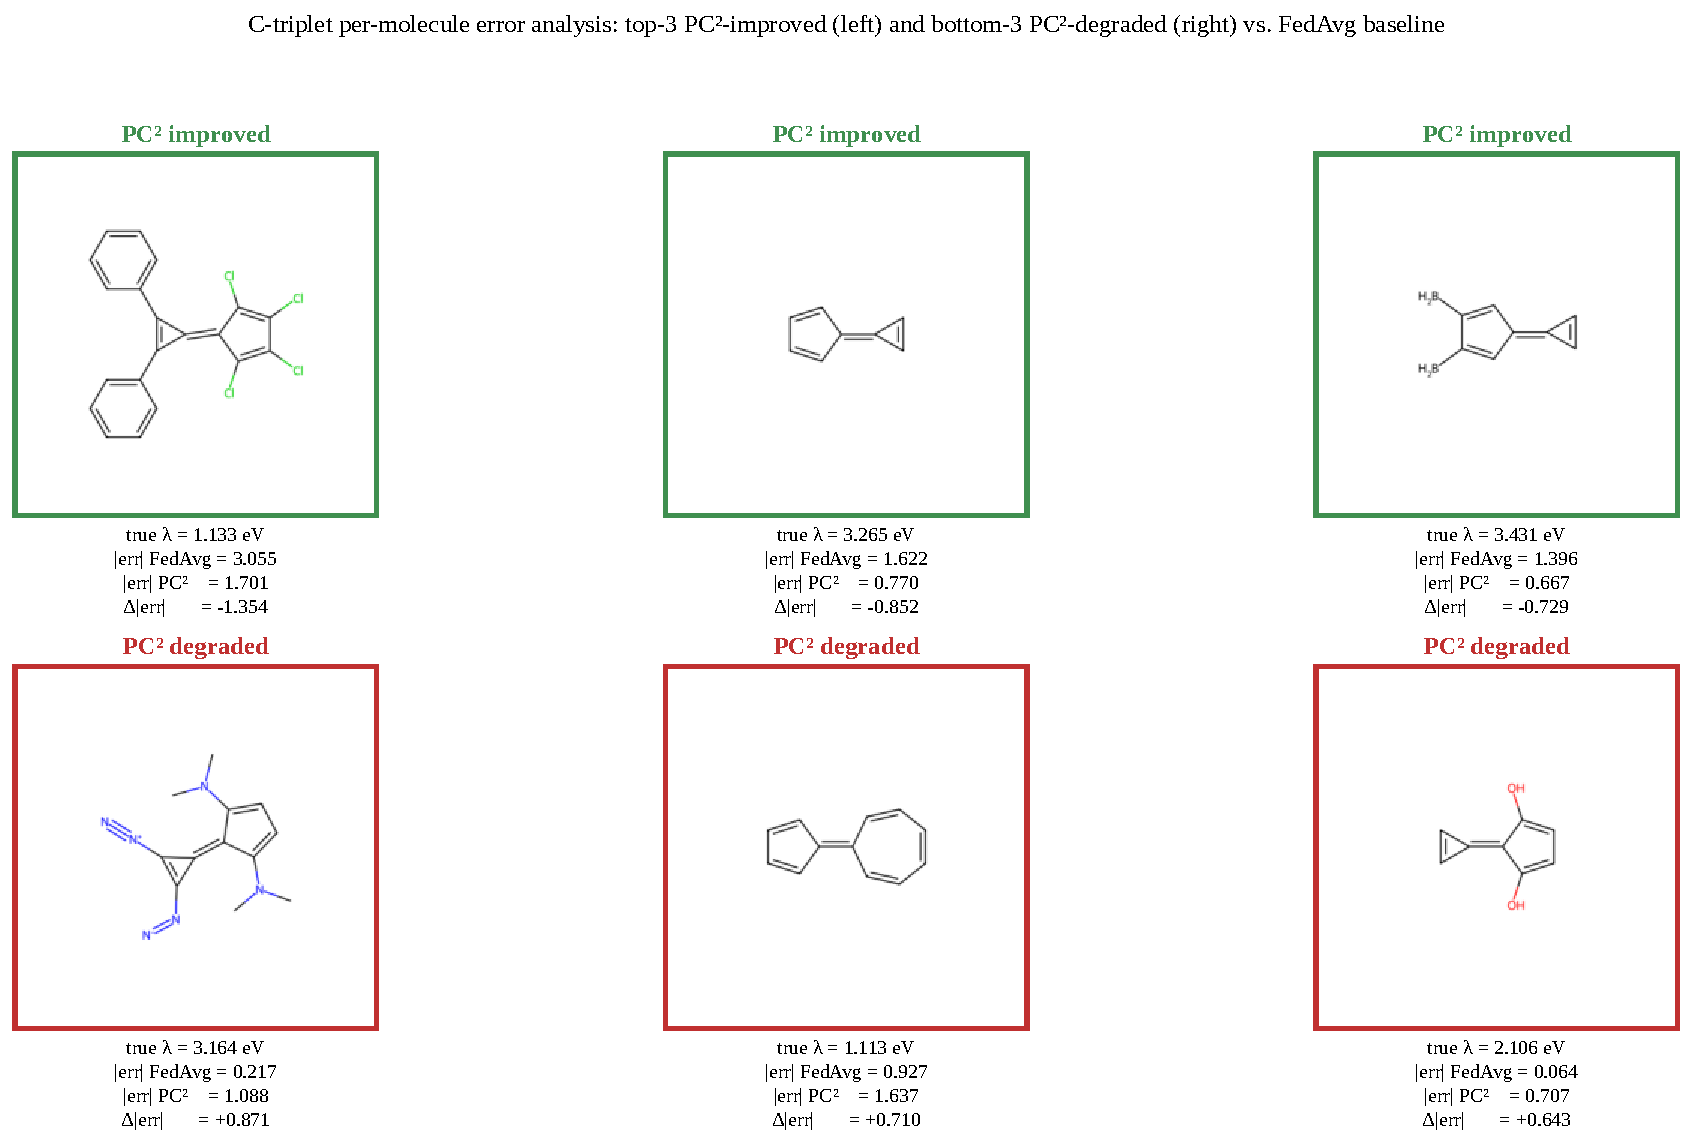
\includegraphics[width=\textwidth]{../figures/FigS1_per_molecule_cases.pdf}
\caption[Per-molecule error analysis on C-triplet -- illustrative cases]{\textbf{Figure S1.} Per-molecule error analysis on C-triplet --- illustrative cases. Three molecules where \PC{} achieves the largest reduction in absolute error relative to FedAvg (left column, green outlines) and three where it shows the largest degradation (right column, red outlines), selected by per-molecule $\Delta|\mathrm{err}|$. Per-molecule absolute errors are aggregated as the median across the five seeds. The figure is provided as a qualitative aid for chemistry interpretation only and is \textbf{not} the basis of any statistical claim; the per-molecule rankings can vary across seeds and across choice of baseline. Demoted from main-text Figure 6 to Supporting Information on 2026-05-13.}
\label{fig:si:cases}
\end{figure}

% =============================================================================
\section{Reproducibility checklist}\label{si:repro}

\subsection{Random seeds}
$\{42, 123, 456, 789, 1000\}$.  \verb|set_all_seeds(seed)| initialises \verb|random|, \verb|numpy.random|, \verb|torch.manual_seed|, \verb|torch.cuda.manual_seed_all|, and sets \verb|torch.backends.cudnn.deterministic = True|.

\subsection{Hardware and runtime}
Dual NVIDIA A30 24~GB (CUDA 12.4), dual Intel Xeon Platinum 8260. Each federated run $\approx 30$ minutes wall-clock; the 25-run main batch (5 methods $\times$ 5 seeds) plus the 20-run ablation batch (4 ablations $\times$ 5 seeds) for this manuscript total $\approx 20$ GPU-hours.

\subsection{Code paths}
\noindent\footnotesize
\begin{tabularx}{\textwidth}{@{}X >{\ttfamily}l@{}}
\toprule
\normalfont Component & \normalfont Path \\
\midrule
Data loading and graph construction            & src/data\_utils.py \\
Encoders, heads, adapter, calibration          & src/models.py \\
Federated aggregation operators                & src/federated.py \\
Per-round training, evaluation, paired metrics & src/train\_eval.py \\
Transferability matrix construction            & src/transferability.py \\
Experiment registry                            & experiments/configs.py; experiments/run\_all.py \\
5-seed batch driver (E60--E63, E66)            & experiments/run\_pc2\_multiseed.py \\
Ablation batch driver (E65, E68, E69, E70)     & experiments/run\_phase5\_step3\_4.py \\
Paired statistical tests                       & experiments/run\_phase5\_step5\_stats.py \\
Figure and table generation                    & paper/make\_figures.py \\
\bottomrule
\end{tabularx}\normalsize

\subsection{Result files}
See main manuscript Data and Code Availability. Per-molecule predictions and paired stats are persisted under \texttt{results/}.

\subsection{Unit tests}
93 unit tests across four modules pass on the commit hash recorded in \texttt{logs/pc2\_batch1/FROZEN\_INFO.txt}.

\subsection{Transferability JSON invariants}
After Phase 1, the compiled \texttt{T\_transferability.json} satisfies: diag($T_{\mathrm{repr}}$) = diag($T_{\mathrm{adapter}}$) = diag($T_{\mathrm{head}}$) = 1; $T_{\mathrm{head}}[\mathrm{D}, \mathrm{C\text{-}hole}] = T_{\mathrm{head}}[\mathrm{D}, \mathrm{C\text{-}triplet}] = 0$; $T_{\mathrm{head}}[\mathrm{C\text{-}hole}, \mathrm{C\text{-}triplet}] = T_{\mathrm{head}}[\mathrm{C\text{-}triplet}, \mathrm{C\text{-}hole}] = 0$. SHA-256 recorded in \texttt{FROZEN\_INFO.txt}.

% =============================================================================
\section{Additional limitations and future work}\label{si:lim}

\subsection{Deferred baselines}
MOON~\citep{Li2021_MOON} and D-MPNN / ChemProp~\citep{Yang2019_ChemProp} are recommended additions for a manuscript revision.

\subsection{Learnable calibration}
A learnable affine layer over the standardised output (E72 ablation, planned) was deferred to avoid introducing additional degrees of freedom at the present sample size.

\subsection{C-hole data ceiling}
All evaluated methods produce MAE in the narrow band \SI{0.368}{}--\SI{0.414}{\eV} on $n = 53$ C-hole LOOCV, with no paired test reaching significance. Expanding C-hole through additional $\omega$B97X-D conformer-resolved measurements is the most direct route to breaking the ceiling.

\subsection{Chemistry gate testing under more diverse client pairs}
$T_{\mathrm{repr}}$ between C-hole and C-triplet is near-unity. The chemistry-driven encoder gate is therefore tested on the easier regime (very similar chemistry) but not on the harder regime (moderate diversity).

\subsection{Font availability for current draft figures}
The figures distributed with this manuscript draft were rendered using Liberation Serif (a metric-compatible substitute for Times New Roman) because Times New Roman was not installed on either of the project's compute nodes at the time of writing. For final journal submission, the figure-generation script (\texttt{paper/make\_figures.py}) should be re-run on a machine that has Times New Roman registered with matplotlib's font manager.

\subsection{Other future directions}
Quantity-aware multi-head extensions; communication compression via top-$k$ sparsification; federated active learning using the per-task-client $\sigma$ as an uncertainty proxy.

% =============================================================================
\section{Controlled pseudo-federation tests of task-specific calibration}\label{si:calgen}

To check whether the calibration signal observed on the real TADF C-triplet target (\S\ref{si:abl-e71}, main-text Figure~5) is an isolated outcome or part of a broader pattern, we ran two additional controlled experiments on synthetic pseudo-federations constructed from the public QM9-derived dataset \texttt{data/client\_a\_b/public\_reorg\_energy\_15210.csv}. \textbf{These experiments do not modify any main-text result on the real C-hole or C-triplet targets}; the raw outputs are in \texttt{results/calibration\_generalization/} and the unified report is at \texttt{paper/calibration\_generalization/calibration\_generalization\_report.md}. The summary verdict is PASS-LIMITED: calibration generalises in the small-target regime that mirrors C-triplet, but not in the moderate-target / aggressive-transform regime where local-only training is already adequate.

\subsection{Phase 1 -- label-scale stress test}
A five-client pseudo-federation was built with one target (S1, identity label transform, $n_{\mathrm{target}} = 100$) and four sources carrying aggressive affine plus noise transforms (S2: $y \to 2y + 0.5$; S3: $y \to 0.5y - 0.2$; S4: $y \to 3y + 1.0$; S5: $y + \mathcal{N}(0, 0.05)$, $n_{\mathrm{source}} = 200$ each). Five seeds, twelve communication rounds, five local epochs per round. Across the five seeds, local-only training reaches MAE $= 0.309 \pm 0.010$~eV (mean $\pm$ SEM); plain FedPer reaches $0.358$; FedPer~$+$~calibration reaches $0.340$; FedAvg without calibration reaches $0.342$. Paired Wilcoxon on per-target median-across-seeds absolute errors: \textbf{FedPer~$+$~calibration vs.\ FedPer: $\Delta$MAE $= +0.010$~eV ($p = 0.73$, n.s.)} -- calibration shows no advantage over plain FedPer at this $n_{\mathrm{target}}$. FedPer~$+$~calibration vs.\ FedAvg without calibration: $\Delta$MAE $= -0.043$~eV ($p = 0.008$) -- calibration improves over no-encoder-personalisation. Local-only is already competitive in this regime, so the federation itself is not load-bearing.

\subsection{Phase 2 -- pseudo-task multi-target validation}
Ten label-quantile-binned pseudo-targets ($n_{\mathrm{per\;task}} = 50$, identity transforms) were each evaluated under the same federation. Three seeds, eight communication rounds, three local epochs per round, three folds of CV per target. The headline result is that \textbf{FedPer~$+$~calibration improved over plain FedPer on 9 of 10 pseudo-targets}, with median $\Delta$MAE $= -0.020$~eV (interquartile range $[-0.030, -0.013]$). Per-task paired Wilcoxon tests give $p < 0.001$ on 7 of 10 tasks; one task is borderline ($p = 0.745$ on T00\_quantile0, $\Delta$MAE $= -0.001$~eV) and one is in the opposite direction (T09\_quantile9, the extreme high-label quantile, $\Delta$MAE $= +0.035$~eV, $p = 0.112$). This supports the calibration-centered interpretation in small-target pseudo-federations.

\subsection{Phase 3 -- calibration variants (not run)}
Shrinkage calibration and learnable affine calibration were specified as candidate variants but not executed (\texttt{results/calibration\_generalization/calibration\_variants/variant\_feasibility\_report.md}); the PASS-LIMITED Phase 1 result does not meet the threshold for full variant testing. Shrinkage would not require a \texttt{src/} modification; learnable affine would, and at $n \approx 30$ LOOCV-train labels carries a substantial over-fit risk. The feasibility report records the decision and the design space.

\begin{table}[ht]
\centering\small
\caption{Calibration-generalisation experiments. Controlled pseudo-federation tests built from public QM9-derived data; \textbf{not} real TADF targets. ``Comparison'' rows are paired Wilcoxon signed-rank tests on per-target median-across-seeds absolute errors.}\label{tab:calgen}
\begin{tabular}{lllllll}
\toprule
Experiment & Setting & $n_{\mathrm{target}}$ & Comparison & $\Delta$MAE (eV) & Wilcoxon $p$ & Outcome / interpretation \\
\midrule
Phase 1 label-scale stress  & 5 clients, aggressive transforms & 100 & cal vs.\ FedPer    & $+0.010$ & $0.73$  & no advantage over FedPer in this regime \\
Phase 1 label-scale stress  & 5 clients, aggressive transforms & 100 & cal vs.\ FedAvg    & $-0.043$ & $0.008$ & improves over FedAvg (no encoder personalisation) \\
Phase 2 pseudo-task val.    & 10 label-quantile pseudo-targets  &  50 & cal vs.\ FedPer    & median $-0.020$ & 7/10 $< 0.001$ & improves 9/10 pseudo-targets \\
Phase 3 calibration variants & shrinkage / learnable affine     & --- & not run            & ---      & ---     & feasibility report only \\
\bottomrule
\end{tabular}
\end{table}

\paragraph{Summary.}
These controlled experiments strengthen the interpretation that task-specific calibration is useful in small-target heterogeneous settings, while the Phase 1 null result prevents a universal performance claim. We therefore present them as robustness evidence for the small-target reading of the main-text C-triplet result rather than as a claim of general superiority.

% =============================================================================
\bibliography{references}

\end{document}
